%%%%%%%%%%%%%%%%%%%%%%%%%%%%%%%%%%%%%%%%%%%%%
%\documentclass[useAMS,usenatbib,usegraphicx,referee]{mn2e}
\documentclass[useAMS,usenatbib,usegraphicx]{mn2e}
%\documentclass{emulateapj}
\usepackage{times,amssymb,hyperref,aas_macros}
\usepackage{comment}

%%%%%%%%%%%%%%%%%%%%%%%%%%%%%%%%%%%%%%%%%%%%%

\newcommand{\dmdt}{$\Delta$m-$\Delta$t}
\newcommand{\dfdt}{$f_{\rm min}$-$\Delta$t}
\newcommand{\dt}{$\Delta$t}

\begin{document}

\title[The transiting dust clumps of RZ~Psc]{The transiting dust clumps in the evolved
  disk of the Sun-like UXOr RZ~Psc}

\author[Grant M. Kennedy et al]{Grant M. Kennedy\thanks{Email:
    \href{mailto:gkennedy@ast.cam.ac.uk}{gkennedy@ast.cam.ac.uk}}$^1$,
  Matthew A. Kenworthy$^2$,
  Joshua Pepper$^3$, \newauthor
  Joseph E. Rodriguez$^{4,5}$, 
  Robert J. Siverd$^6$, \&
  Keivan G. Stassun$^{5,7}$ \\
  $^1$ Institute of Astronomy, University of Cambridge, Madingley Road, Cambridge CB3
  0HA, UK \\
  $^2$ Leiden Observatory, Leiden University, PO Box 9513, NL-2300 RA Leiden, the
  Netherlands \\
  $^3$ Department of Physics, Lehigh University, 16 Memorial Drive East, Bethlehem, PA
  18015, USA \\
  $^4$ Harvard-Smithsonian Center for Astrophysics, 60 Garden Street, MS-78, Cambridge, MA
  02138, USA \\
  $^5$ Department of Physics and Astronomy, Vanderbilt University, 6301 Stevenson Center,
  Nashville, TN 37235, USA \\
  $^6$ Las Cumbres Observatory Global Telescope Network, 6740 Cortona Dr., Suite 102, Santa
  Barbara, CA 93117, USA \\
  $^7$ Department of Physics, Fisk University, 1000 17th Avenue North, Nashville, TN
  37208, USA \\
}
\maketitle

\begin{abstract}
  RZ~Psc is a young Sun-like star, long associated with the UXOr class of variable stars,
  that is occulted by optically thick dust clumps several times each year. The system has
  an infrared excess, interpreted as evidence that the dimming events are the passage of
  asteroidal fragments in front of the host star. Here, we present a decade of optical
  photometry of RZ~Psc and take a critical look at the asteroid belt interpretation. We
  find weak evidence for periodicity near 65 days (0.3au), and show that the distribution
  of light curve gradients is non-uniform for deep events, which we interpret as possible
  evidence for an asteroidal fragment-like clump structure. However, the clumps are very
  likely seen above a high optical depth mid-plane, so the disk's bulk clumpiness is not
  revealed. While circumstantial evidence suggests an asteroid belt is more plausible
  than a gas-rich transition disk with an inner hole, the evolutionary status remains
  uncertain. We suggest that the rarity of Sun-like stars showing disk-related
  variability may arise because i) any accretion streams are transparent, and/or ii)
  turbulence above the inner rim is normally shadowed by a flared outer disk.
\end{abstract}

\begin{keywords}
  circumstellar matter, variable stars, protoplanetary disks, debris disks
\end{keywords}

\section{Introduction}\label{s:intro}

Disks of gas and dust surround essentially all young analogues of our Sun
\citep[e.g.][]{2001ApJ...553L.153H}. The lifetime of the gas in these disks is very short
compared to the stellar lifetime, and within a few million years most has accreted onto
the star and the remainder been lost to space in photoevaporative flows. The evolution of
the dust during this phase is uncertain, but the existence of gas giant planets makes it
clear that planetary building blocks, and of course some planets, form on a similar or
shorter timescale.

Beyond the first few million years a typical star hosts a planetary system, the
components being the planets themselves and a residual disk of small bodies. These
``planetesimals'' -- the asteroids and comets -- make up the ``debris disk'', where the
standard picture is that destructive collisions between them generate a size distribution
of fragments that extends down to micron-sized dust
\citep[e.g.][]{1993prpl.conf.1253B,2002MNRAS.334..589W,2010RAA....10..383K}.

The state of planetary systems as they emerge from the gas-rich phase is
uncertain. Planets' locations are not finalised at this epoch, but may move by
interacting with other stars, planets, and/or planetesimals in the system
\citep[e.g.][]{2007ApJ...669.1298F,1996Sci...274..954R,2005Natur.435..459T}. Similarly,
the state and origin of the debris disk is uncertain. At stellocentric distances near
1au, the region of interest in this article, it could be that dust observed at this time
is related to the final stages of planet formation
\citep[e.g.][]{2010ApJ...717L..57M,2012MNRAS.tmp.3462J}, originates in young analogues of
our Asteroid belt \citep{2013MNRAS.433.2334K}, is a signature of comets scattered inwards
from more distant regions \citep[e.g.][]{2009MNRAS.399..385B}, or is simply a remnant of
the gas-rich disk that has yet to be dispersed \citep{2014MNRAS.tmp...88K}. In the
absence of gas detections that argue for the latter scenario, discerning among these
various scenarios, which are not mutually exclusive, is difficult.

A promising way to probe these inner regions is by observing temporal variability
\citep[e.g.][]{2014Sci...345.1032M}. Optical and IR stellar variation has been studied
for decades \citep[e.g.][]{1945ApJ...102..168J,1994AJ....108.1906H}, and has recently
been reinvigorated by large scale efforts
\citep[e.g.][]{2011ApJ...733...50M,2014AJ....147...82C} and as a side-effect of
large-scale surveys for transiting planets
\citep{2012AJ....143...72M,2013AJ....146..112R,2016MNRAS.457.3988B}. Of many different
classes of variables, the ones of most interest and relevance here are the
``UXOrs''. These are usually Herbig Ae/Be stars, and typically show several magnitudes of
extinction that is generally attributed to variable obscuration by circumstellar dust
\citep{1994AJ....108.1906H,1999AJ....118.1043H,2000A&A...364..633N}.\footnote{Not all
  stars occulted by dust are UXOrs. Two main classes are: those occulted by circumstellar
  material beyond $\gtrsim$10au, such as AA~Tau and V409~Tau which show
  $\gtrsim$year-long dimming events \citep{2013A&A...557A..77B,2015AJ....150...32R}, and
  systems such as $\epsilon$~Aur, J1407, EE~Cep, and OGLE-LMC-ECL-11893 where the
  occultations are attributed to circumsecondary disks
  \citep[e.g.][]{1999MNRAS.303..521M,2012AJ....143...72M,2014ApJ...788...41D,2015ApJS..220...14K}.}
Two key arguments that favour circumstellar dust as the cause are i) ``blueing'', where
the star is reddened when moderately dimmed but returns to the stellar colour for very
deep ($\gtrsim$1mag) events -- the remaining flux is interpreted as light scattered off
circumstellar dust \citep{1988SvAL...14...27G}, and ii) increased polarisation fraction
during dimming events, caused by a greater fraction of the flux being contributed by
dust-scattered light \citep[e.g.][]{2001ARep...45...51R}. UXOrs therefore reveal
information on the degree of non-axisymmetry, the ``clumpiness'', of dust orbiting a star
on spatial scales similar to the star itself. The observations can span multiple orbits
to test for repeated dimming events \citep[e.g.][]{1999A&A...349..619B}, and by using
different bandpasses and polarisation can estimate dust grain sizes
\citep[e.g.][]{1988SvAL...14...27G,1994ASPC...62...63G}.

In the majority of UXOr-like cases (i.e. those related to obscuration by dust), including
other classes such as ``dippers''
\citep[e.g.][]{2014AJ....147...82C,2016ApJ...816...69A}, the processes causing young
stars to vary are attributed to gas-rich protoplanetary disks. For Herbig Ae/Be stars the
obscuration is thought to be caused by hydrodynamic turbulence that lifts dust above the
puffed up inner rim of a self-shadowed disk \citep{2003ApJ...594L..47D}. For the dippers,
which are observed around low-mass stars, the obscuration is attributed to dust in
accretion streams that link the inner disk and the stellar surface, and/or to variations
in the height of the inner disk edge
\citep{1999A&A...349..619B,2016ApJ...816...69A,2016arXiv160503985B}. The common theme is
therefore that the location of the occulting dust is as close to the star as physically
possible, being set by sublimation. These systems tell us about the nature of turbulence
and accretion in gas-dominated disks, but so far reveal little about how these disks
transition to the debris phase and the subsequent evolution.

Here we focus on RZ~Psc, a star that shows UXOr-like variability
\citep[e.g.][]{1985PZ.....22..181Z,1999A&AS..140..293G,2003ARep...47..580S}. As a young
K0V type star with no evidence for gas accretion, but a strong infrared (IR) excess
suggestive of an Asteroid belt analogue, this system appears unique among UXOrs and may
provide new information on the structure of inner planetary systems following dispersal
of the gas disk \citep{2010A&A...524A...8G,2013A&A...553L...1D}. Specifically, we use a
decade of ground-based optical photometry of RZ~Psc (section \ref{s:data}) to draw
conclusions on dust location (section \ref{s:where}), and discuss the possible disk
structure and evolutionary state in section \ref{s:disk}. We conclude in section
\ref{s:conc}.

\section{A clumpy dust ring near 0.5 au?}\label{s:rzpscintro}

There is significant evidence that the optical variations seen towards RZ~Psc are caused
by circumstellar dust: i) during dimming events the colour becomes redder
\citep{1985PZ.....22..181Z,1980PZ.....21..310K} in a way consistent with that expected
for dust \citep{1981Afz....17...87P,2004ARep...48..470P}, ii) the maximum depth is about
2.5mag and during these events the colour returns to near stellar values, suggesting that
the remaining emission is from light scattered off the circumstellar dust \citep[i.e. the
star is fully occulted,][]{1981Afz....17...87P,1988SvAL...14...27G}, and iii) the
polarisation fraction increases during the transits, as expected if an increasing
fraction of the light is scattered off circumstellar dust
\citep{1988SvAL...14...27G,1991Afz....34..333K,2003ARep...47..580S}.

What separates RZ~Psc from other UXOrs (and dippers) is i) the spectral type is K0V
rather than Herbig Ae/Be for UXOrs and M-type for dippers, ii) the occulting dust lies
well beyond the sublimation radius, and iii) the star is not associated with a
star-forming region so is inferred to be a few tens of millions of years old. The dust
distance has been inferred from the speed of ingress of dimming events, which was
previously estimated as about 0.6au \citep[for circular
orbits,][]{2013A&A...553L...1D}. Corroborating evidence comes from the $\sim$500K
temperature of the dust seen in the mid-IR, which places it near 0.4-0.7au (depending on
optical depth) and therefore at a location consistent with the occulting dust
\citep{2013A&A...553L...1D}. The distance to RZ~Psc is unknown, but as an apparently
isolated star that shows Li absorption the age has been estimated as a few tens of Myr,
and therefore beyond the age at which a gas-rich disk should exist
\citep{2010A&A...524A...8G,2014A&A...563A.139P}. Further distinguishing features are that
the duration of the dimming events is relatively short compared to other UXOrs, a few
days rather than a few weeks, and that no near-IR excess or accretion signatures are seen
\citep{2014A&A...563A.139P}, so interpretations related to accretion of disk material
onto the star \citep[e.g.][]{1999AJ....118.1043H,1999A&A...349..619B,2016arXiv160503985B}
are unlikely.

Thus, the potentially compelling and unique aspect for RZ~Psc is that we are observing
dimming events from dust in a main-sequence planetary system that resides at about
0.5au. This dust is also seen in thermal emission, so deriving joint constraints on the
dust properties and structure may be possible. As argued by \citet{2013A&A...553L...1D} a
picture is emerging in which RZ~Psc is surrounded by a massive young version of our own
asteroid belt, in which planetesimals are continually being destroyed. These collisions
generate the large collective surface area of small dust that emits strongly in the
mid-IR, and the system geometry means that this dust also sometimes passes in front of
the star.

Given an interpretation related to individual planetesimal disruptions, rather than
hydrodynamics, it is perhaps surprising that to date the dimming events are not seen to
be periodic \citep{1999AstL...25..243R,2013A&A...553L...1D}. The only cyclical variation
seen in light curves for RZ~Psc is a 12.4 year variation with an amplitude of 0.5 mag,
which is attributed to either a magnetic cycle, or precession of an otherwise unseen
outer disk due to perturbations from an unseen companion \citep{2013A&A...553L...1D}.

\section{Time series photometry}\label{s:data}

% yearly-lc.pro
\begin{figure*}
  \begin{center}
    \hspace{-0.5cm} 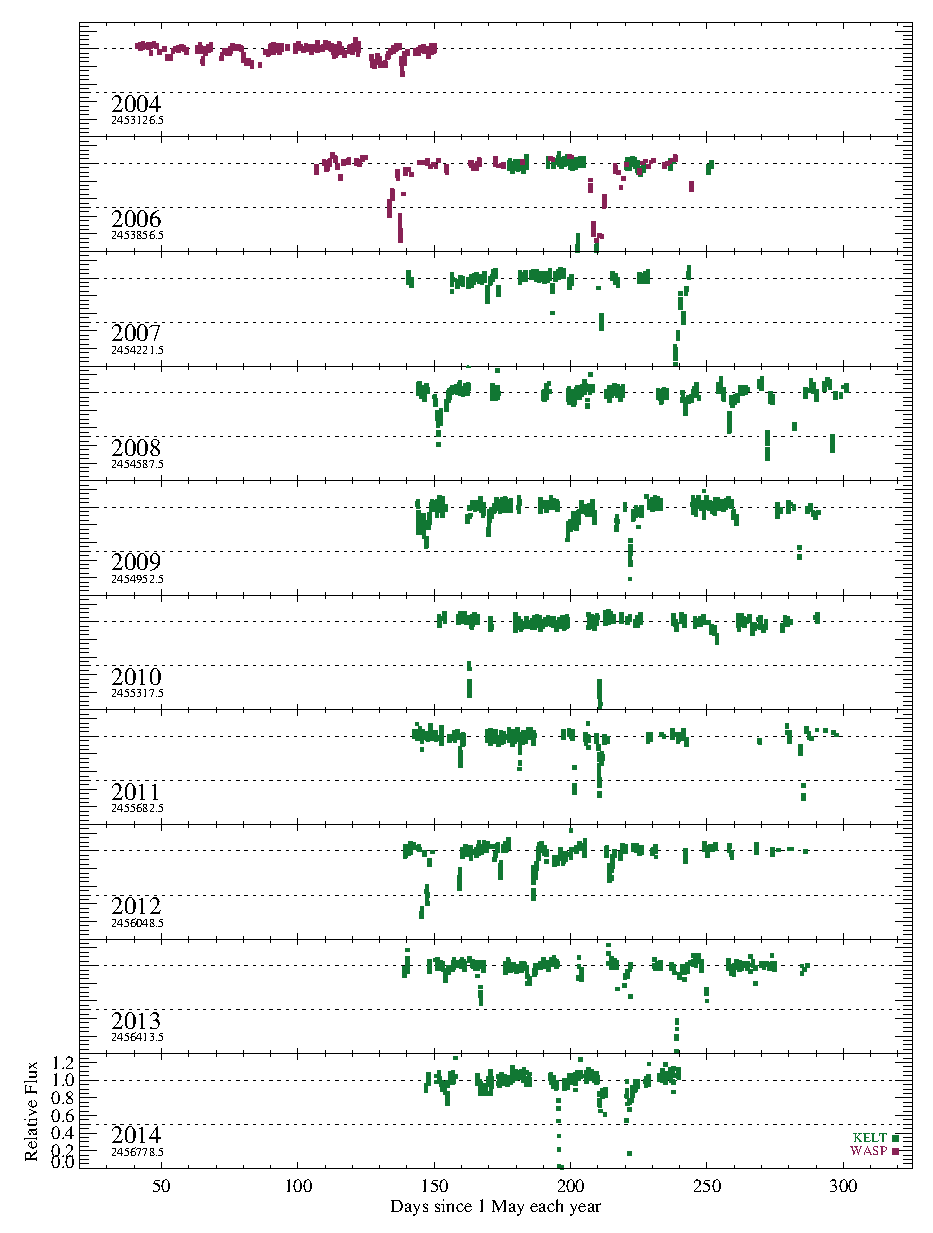
\includegraphics[width=\textwidth]{figs/yearly-2004.eps}
    \caption{WASP and KELT-North data.}\label{fig:waspkelt}
  \end{center}
\end{figure*}

To study the temporal variability of RZ~Psc we use two seasons of public data from the
Wide-Angle Search for Planets \citep[WASP,][]{2006PASP..118.1407P}, and nine seasons of
data from the Kilodegree Extremely Little Telescope North
\citep[KELT-North,][]{2007PASP..119..923P}. We also collected, but ultimately did not
use, photometric observations of RZ~Psc from a wide variety of other sources \citep[][,
the Catalina Sky Survey, the American Association of Variable Star Observers, the All-Sky
Automated
Survey]{1994AJ....108.1906H,1973IBVS..783....1K,1980PZ.....21..310K,1985PZ.....22..181Z,1991Afz....34..333K,1997AcA....47..467P,2014Ap.....57..491P}. Most
of these other data have been previously published and their collation here is largely
for the benefit of others. This compilation contains nearly all data for which tables
have been published, but aside from the Harvard plate photometry published by
\citet{1999A&AS..140..293G} we have not sought other photometry so the light curve
remains incomplete.\footnote{Normalised photometry is available at
  \href{https://github.com/drgmk/rzpsc}{https://github.com/drgmk/rzpsc}}

Here we focus on the WASP and KELT-North data, as it has not been previously analysed and
has considerably higher cadence (many measurements per night) and temporal coverage
(nightly, weather permitting) than other data sets. The WASP data from 2004 and 2006 are
public and were obtained from an online
archive\footnote{\href{http://wasp.cerit-sc.cz}{http://wasp.cerit-sc.cz}}. These data
were processed in a manner similar to that described by \citet{2014MNRAS.441.2845V},
where common-mode variations were removed using 50 quiet nearby stars. The KELT-North
data, 2006-2014, were used in raw form, the only specific treatment being a 4\% relative
correction being made to ensure observations taken in the ``east'' and ``west'' telescope
orientations have the same calibration. For a full description of the KELT-North data
reduction, see \citet{2012ApJ...761..123S}.

We normalised each year's data from each instrument separately by converting magnitudes
to flux density and dividing out the sigma-clipped median. In doing so we are assuming
that variations due to the slightly different filter bandpasses are unimportant. We
normalise the light curve to have an out-of-occultation baseline of 1 (Figure
\ref{fig:waspkelt}). Each row shows a season's data, starting on May 1 each year (JD also
indicated). Most year's data therefore extend into the next year, so the ``2006 data''
refers to data from the 2006/2007 observing season.

\subsection{Qualitative light curve overview}\label{ss:quallc}

% yearly-zoom.pro
\begin{figure*}
  \begin{center}
    \hspace{-0.5cm} 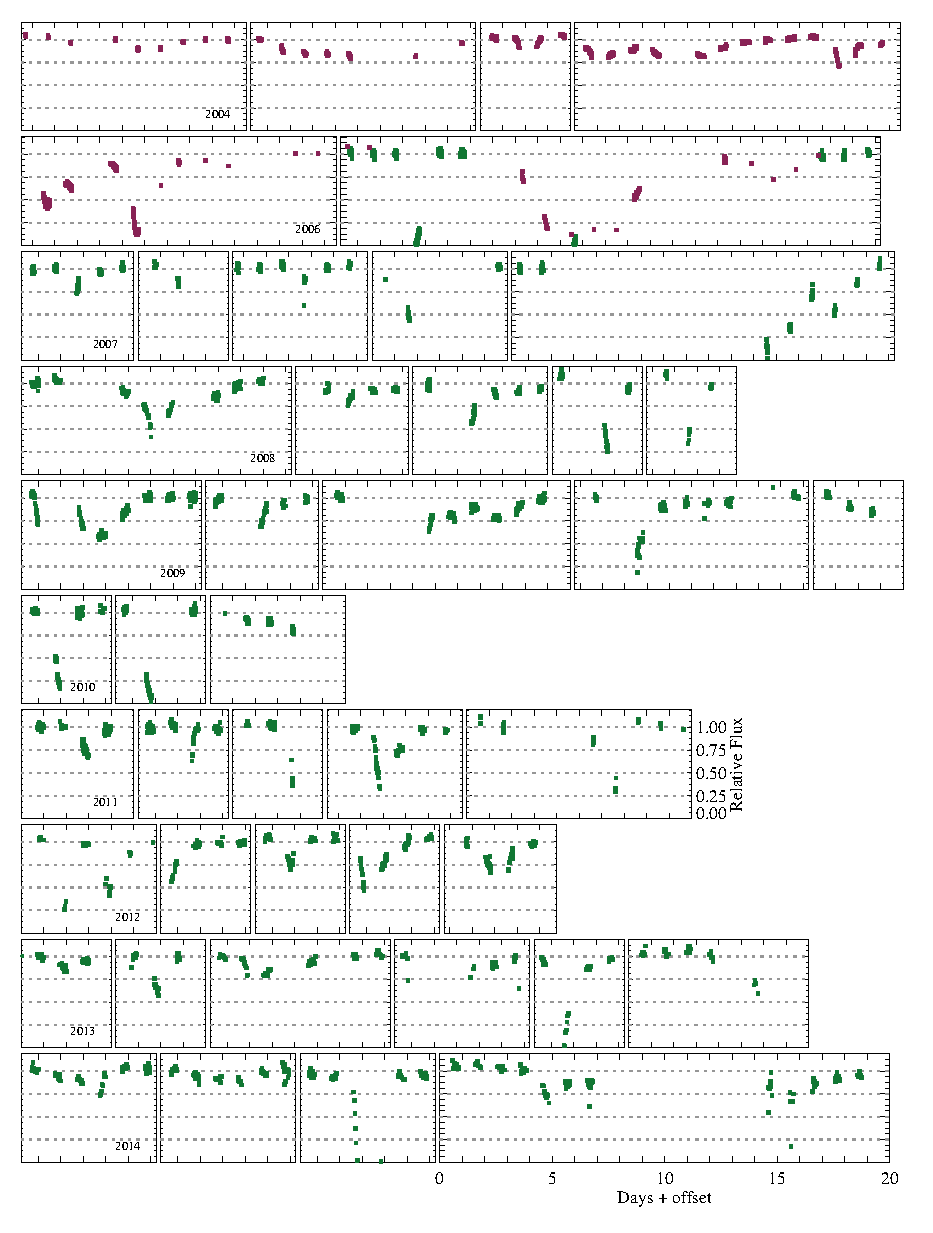
\includegraphics[width=\textwidth]{figs/yearly-zoom.eps}
    \caption{WASP and KELT-North data, focussing on dimming events. The vertical and
      horizontal scales in each sub-panel are the same.}\label{fig:waspkeltzoom}
  \end{center}
\end{figure*}

It is clear from Figure \ref{fig:waspkelt} that RZ~Psc undergoes the very deep dimming
events that are typical of UXOrs. These are seen a few times each observing season and
vary in complexity, with a few extended events (e.g. 2006) and a greater number of
``neater'' single events (e.g. 2010). In some years there is also significant variability
at shallower depths. Of particular note is the pair of deep events in 2006; these appear
to be about 70 days apart, and given the suggestion that the asteroid belt analogue
resides near 0.5au a natural inference is that these two events are related. If true,
this repetition corresponds to a semi-major axis of about 0.3au, which given
uncertainties in the true disk spectrum could be consistent with the location of the
asteroid belt. In 2004 there are about 100 days of near-consecutive nights of data and no
deep events, so either the true period is longer than 100 days, or dust clumps can be
created (and perhaps destroyed) on timescales of a year or so.

In Figure \ref{fig:waspkeltzoom} we have selected most of the events from each year and
shown them at a greater temporal resolution. The scale in each panel is the same, so
wider boxes simply cover longer events. Most events appear to last at least a few days,
suggesting that only having nightly coverage does not seriously hinder our ability to
detect most events. However, the events are sufficiently short and irregular that the
true shape of events remains uncertain. While it is likely that interpolation of the
photometry for the fourth event in 2011 (that is, the fourth box from the left in the row
corresponding to 2011 in Figure \ref{fig:waspkeltzoom}) would resemble the true light
curve, this assumption seems very unlikely to yield the true evolution of more complex
events like those in 2006.

Nevertheless, Figure \ref{fig:waspkeltzoom} shows an unprecedented view of dimming events
seen towards RZ~Psc, and that key information on the ingress and egress of dimming events
is present. The dimming rate is such that it can be resolved temporally, and hence the
velocity and radial location of the dust clumps estimated. While such estimates have been
made in the past based on one or two individual events \citep{1985PZ.....22..181Z}, these
data make them possible for an ensemble of tens of events.

\section{Where are the occulting bodies?}\label{s:where}

The main part of our analysis concerns attempts to extract information from the light
curves, taking advantage of the great number of dimming events seen over ten seasons. In
this section we focus on the radial location of the bodies (``clumps'') that pass in
front of RZ~Psc, first searching for periodicity associated with repeat events, and then
using the light curve gradients to constrain the projected velocities. This analysis
primarily focusses on what can be gleaned from the light curves, and the implications of
these results for different clump origins are then explored in section \ref{s:disk}.

\subsection{Search for periodic dimming events}\label{ss:per}

We begin by estimating the lifetime of an occulting clump as a check on the plausibility
that dimming events should repeat. The rate at which clumps are sheared out is
$dv/dr = - \Omega/2$, which accounting for shear in both forward (interior) and backward
(exterior) directions is to first order ($R_{\rm cl} \ll a$)
\begin{equation}\label{eq:shear}
  v_{\rm sh} = R_{\rm cl} \Omega \, ,
\end{equation}
so the clump expansion rate due to shear in units of clump radii is the same as the
orbital frequency. That is, for an orbital period of a year, after one orbit a clump will
be stretched by a factor of $2\pi$ around the orbit, and the optical depth will be $2\pi$
lower (though it may still be optically thick). Thus, clumps that are not gravitationally
bound are expected to have a short lifetime at optical depths that are large enough to
cause detectable dimming events, but could cause repeated dimming events if they are
initially optically thick.

The coverage in an individual season is 100-150 days. Thus, if the occulting material
resides in an asteroid belt closer than $\sim$0.5au, periodicity in the dimming events
may be visible in a single season's data. Longer orbital periods may be visible across
seasons, though the six-month gap between seasons makes unambiguously linking events
harder. Non-detection of periodicity would imply that the data are not sufficient, or
that strict periodicity does not exist. An intermediate possibility is that occultations
happen with a range of periodicities, perhaps reflecting their origin in a radially broad
region, and that discerning this scenario from randomly occurring occultations is not
possible given the data.

In an attempt to find the expected periodicity we tried several approaches. These are
similar in that they aim to quantify whether some feature in the light curve is repeated
again at a later time, but differ in how well they reveal evidence for a periodic
signal. We found no evidence for events that are related from one year to another, so
focus on statistics derived from individual seasons' data (though these are sometimes
combined).

\subsubsection{Autocorrelation}\label{sss:auto}

% period-search.pro
\begin{figure}
\begin{center}
\hspace{-0.5cm} 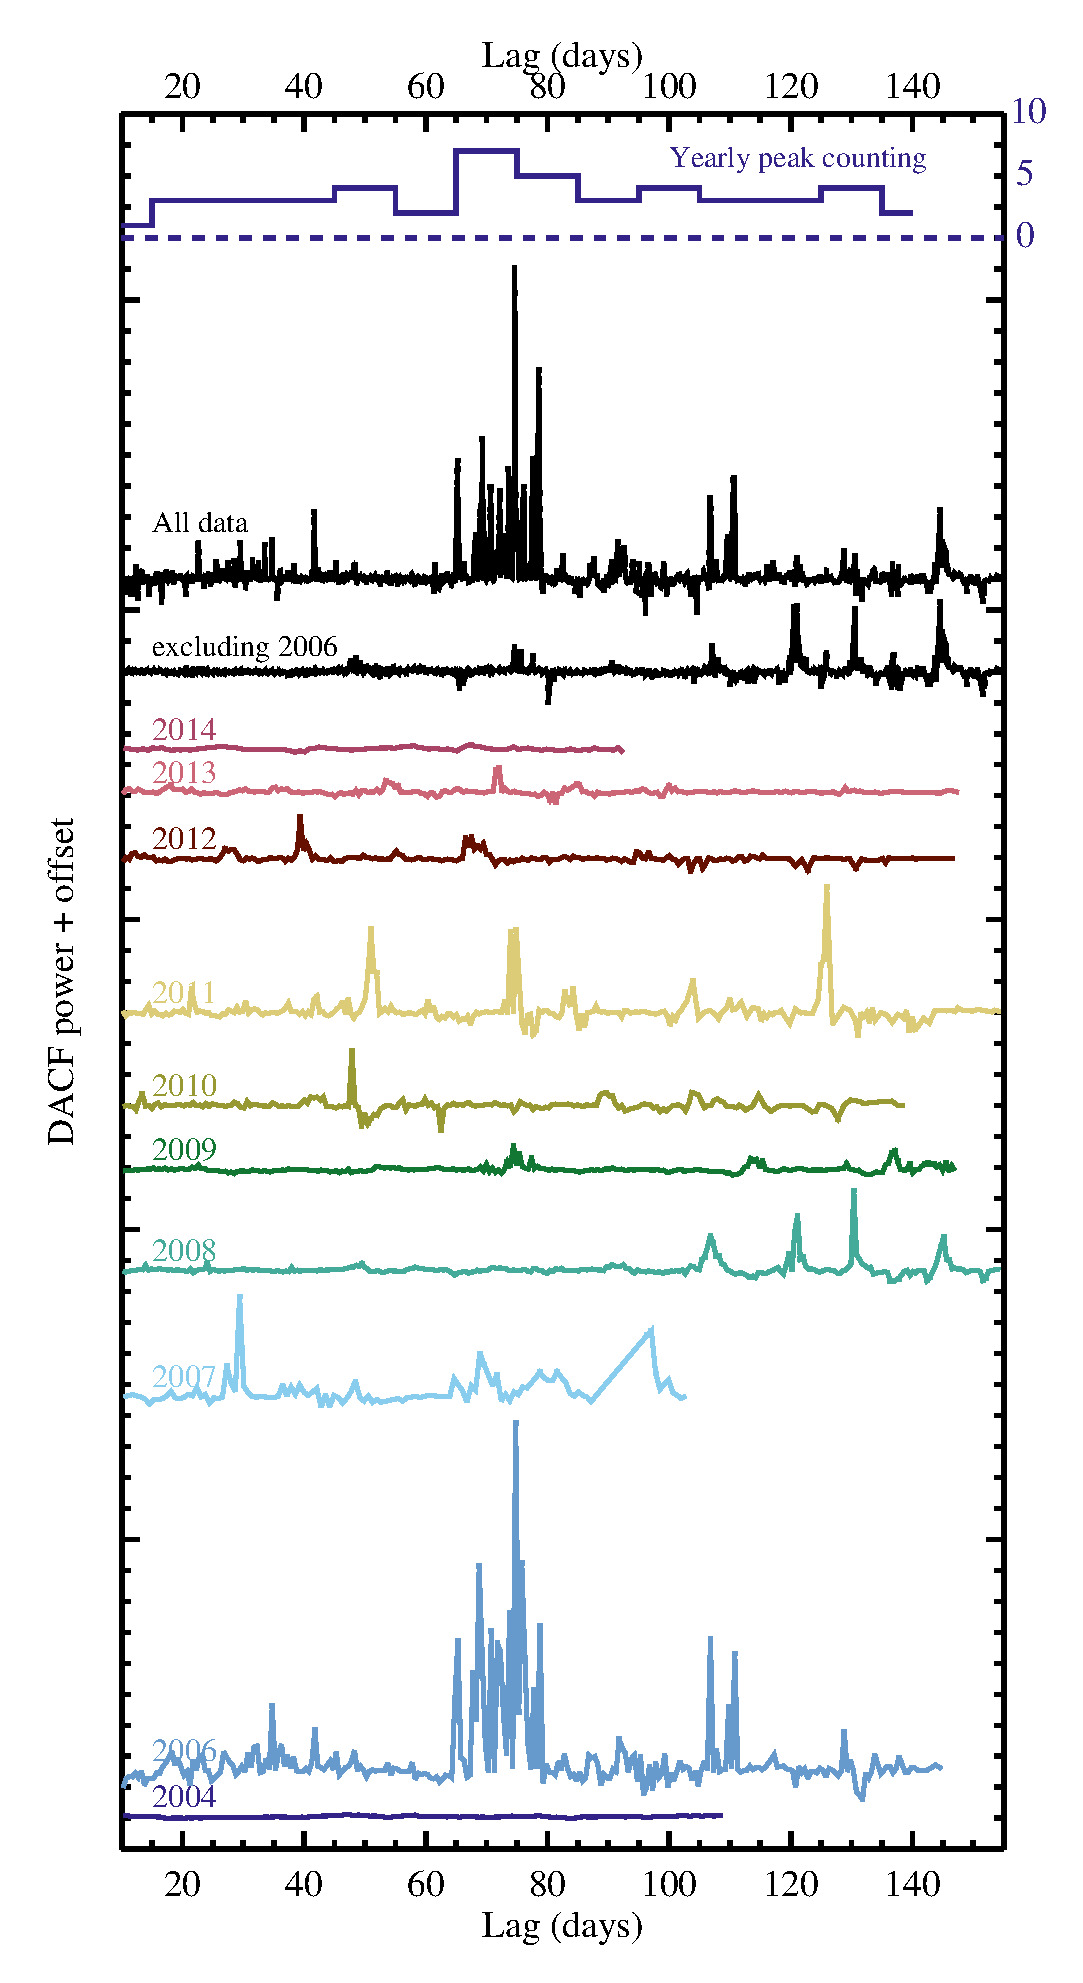
\includegraphics[width=0.5\textwidth]{figs/auto.eps}
\caption{Discrete autocorrelation function for yearly WASP and KELT-North data, computed for
  lags between 10-155 days). The second and third lines from the top show all data, and
  2006-excluded data. Squares show points more than 3$\sigma$ from the sigma-clipped
  mean. The topmost line shows the number of years that show a peak (square) within each
  5 day bin. The peak at 70 days is 7 years and the dashed line is zero.}\label{fig:auto}
\end{center}
\end{figure}

We first used autocorrelation to search for periodicity, rather than methods related to
Fourier transforms (e.g. periodograms). The motivation being that an individual transit
event may be followed by another some number of days later, and perhaps repeat a few
times, but other similarly (but not exactly) separated events may happen years later or
earlier with a phase that is totally different. We therefore used the discrete
autocorrelation function (DACF) proposed by \citet{1988ApJ...333..646E}, though do not
include uncertainties on individual measurements. For a time series with measurements
$a_i$ at times $t_i$ the DACF first computes the mean $\bar{a}$ from the light curve,
here we used the sigma-clipped mean to remove the dimming events. Then for each pair of
points $a_i$, $a_j$ (with $i\ne j$) computes
$U_{ij}=((a_i-\bar{a})(a_j-\bar{a}) / \sigma_a$, with each $U_{ij}$ associated with a
time lag $\Delta t_{ij}=t_j - t_i$. A series of time lags centered at times $t_{rm lag}$
with width $\Delta t_{\rm lag}$ are then used as bins, and the average in each bin is the
DACF. The DACF is not computed for lag bins with no data. The units of the DACF are
standard deviations of the light curve $\sigma_a$ (again calculated using sigma
clipping).

The results are shown in Figure \ref{fig:auto} for time lags (i.e. trial periods) of 10
to 155 days in half-day bins. Comparison of these with the light curves shows that the
DACF recovers most, but not all, events. Conversely, not all DACF peaks are necessarily
associated with real repeat events, as there may of course be multiple distinct clumps
orbiting the star at any given time. Some can be ``swamped'' if a pair of apparent
dimming events comprise only a few measurements, but the temporal sampling of the light
curve elsewhere is sufficiently high. Our attempts to avoid this issue by using
autocorrelation on interpolated data yielded mixed results; heavy filtering, such as
setting all data above a given level to 1, was needed for results similar to the DACF
shown in Figure \ref{fig:auto}.

While several strong peaks appear in the DACF of all data, most of these arise from 2006,
as can be seen in the DACF when these data are excluded. Some peaks remain near 70 days,
as well as at 120 and 145 days, and the latter two could be aliases of periods near 60-70
days, arising simply because an event was missed. That is, the irregular sampling means
that absence of evidence of power at some period in the DACF is not evidence of absence.

The pair of events separated by 70 days in 2006 provides the strongest signal, and most
other years also show events near this period (2007, 2009, 2011, 2012, 2013, 2014). To
illustrate these numbers the topmost line in Figure \ref{fig:auto} quantifies the number
of years that show a peak, in 10 day bins. The peak of 7 years is at 65-75 days, which is
suggestive but not conclusive because a K-S test shows that this distribution is
consistent with being uniform in period.

\subsubsection{Iterative event finding}\label{sss:iter}

In an attempt to avoid some of the difficulties arising from the DACF, we tried a similar
approach that first identifies individual occultation events and then computes the time
delays between them. The main aim was to identify and use all events in a way that avoids
biases related to the sampling of the data and the different relative depths of
potentially repeated events. By repeating this prescription for synthetic data we are
able to test different scenarios for how the occultations do or do not repeat.

For this approach, an event is initially identified as the lowest point that is 6$\sigma$
below the mean, where the mean and standard deviation are again estimated by
sigma-clipping. This lowest point is noted, as are all immediately adjacent points that
are also below the threshold noted. The points so included constitute a single dimming
event. The points belonging to this event are removed from the light curve and the
process repeated until no significant events remain. The time of the event is the time of
the lowest point, and the duration the time between the two end points that are
consistent with the quiescent level. Thus, if an event is in a region of sparse sampling
the duration can appear to be longer than it probably is, though we discard any events
that occur at the beginning or end of an observing season to avoid unreasonably long
events.

For a given set of event times and durations, the range of possible times between events
is then calculated using the maximum allowed by the duration. This calculation is done
for all combinations, yielding $N(N-1)/2$ inter-event time ranges. These ranges are then
``stacked'' into a histogram (i.e. counting +1 for time differences within a given bin)
that shows a measure of the power present at a given time difference.

% plot_lc_dips_dts.py
% \begin{figure*}
  % \begin{center}
  %   \hspace{-0.cm} \includegraphics[width=\textwidth]{figs/lc_dips_dts.ps}
    % \caption{Iterative dimming event finding. The right part of the plot shows the same
    %   time series as Figure \ref{fig:waspkelt}, with the identified dimming events shown
    %   as boxes. The time differences between these events is shown on the left side of
    %   the plot. The boxes are transparent, so the density is a measure of the power at a
    %   given period.}\label{fig:iter}
  % \end{center}
% \end{figure*}

% The results of this procedure are shown in Figure \ref{fig:iter}, which shows the time
% series data, the identified occultations, and the resulting set of periods. At the bottom
% the stacked set of periods shown; allowing each period range plotted to be transparent
% means that the density gives an indication of the power at each period.

The solid lines in Figure \ref{fig:hist} shows this power in histogram form (the same in
each panel), generated from 60 events that were identified in the light curve. The y-axis
should be interpreted as the number of events that are consistent with that period on the
x-axis. As before, there is evidence for a peak, now slightly shifted to near 65 days. In
contrast to the DACF analysis, this power does not all arise from a single year. Most is
contributed by 2004 and 2009, but exclusion of events from these years results in a
similar (but noisier) histogram.

To test what could have been detected, and the quantify the variation in power expected,
we created synthetic light curves with the same temporal sampling as the WASP and
KELT-North data. To do this we set the flux to 1, and randomly injected a number of
dimming events with a flux of 0.1. These events are therefore relatively easy for the
algorithm to detect, but suffer the same sampling issues. We tried individual randomly
occurring events, and periodic events that repeat a fixed number of times. All events
have durations randomly distributed between 1 and 4 days. For random events the remaining
parameter in this model is simply the number of events -- this is the total number over
the 11 year period covered by the WASP and KELT-North data, including when measurements
were not being taken. For repeating events the range of periods and the number of repeats
are additional parameters. To estimate the level of variation in the power spectrum we
repeated the process of injecting synthetic events 500 times, and in each bin estimate
the mean and standard deviation of the power.

% plot_hist_sim.py
\begin{figure}
  \begin{center}
    \hspace{-0.5cm} 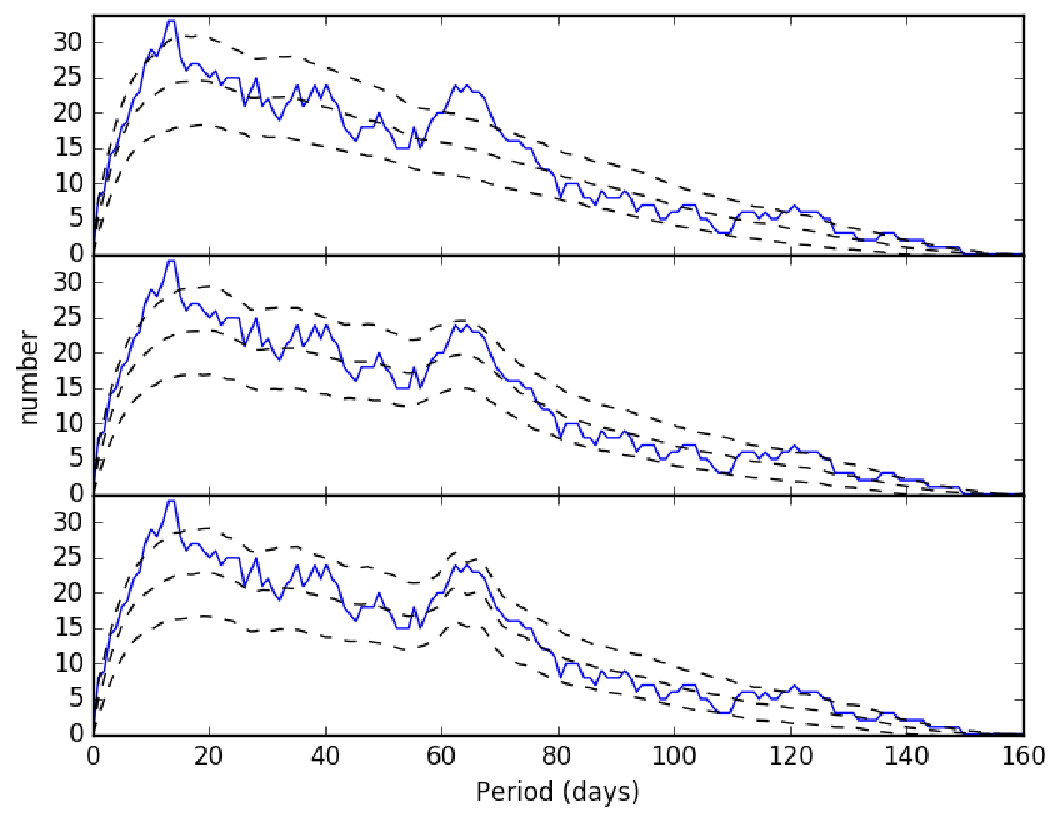
\includegraphics[width=0.5\textwidth]{figs/hist_single.ps}
    \caption{Power at a given period from the iterative event finding. The solid line
      shows the power from the data, and is the same in each panel. The dashed lines show
      the mean and $\pm$1$\sigma$ power from simulated dimming events, which from top to
      bottom are: random, periodic between 64 and 75 days with 3 repeats, and periodic at
      64 days with 10 repeats.}\label{fig:hist}
  \end{center}
\end{figure}

The results are shown in Figure \ref{fig:hist}, where the dashed lines show the mean and
$\pm$1$\sigma$ deviations from the simulations (and solid lines show the data). Each
panel shows a different scenario, from top to bottom these are: 295 random events, 100
events with periods between 64 and 75 days and 3 repeats, and 100 events with a period of
64 days and 3 repeats. The purely random events are marginally disfavoured; while the
data lie outside the dashed lines, these are only 1$\sigma$. Nevertheless, the middle and
bottom panels show that the possible peak near 65 days could be caused by events with a
range of periods, but that only a single period of 64 days is actually needed and yields
a slightly stronger peak. The remaining excess periodicity near 10 days is not accounted
for by any of the models, but could be an indication that on this timescale events are
related (e.g. a clump that has separated into several). That the real signal nearly lies
within the 1$\sigma$ variation expected for randomly occurring events shows that the
evidence for periodicity is weak, but that as found by the autocorrelation analysis, this
weak evidence points towards 64 days as the most likely period.

A side-effect of the simulations is an estimate of about 300 dimming events over the
period between 11 June 2004 and 21 February 2015 (3851 days). This number is five times
larger than the 60 events detected by the iterative search. Thus, an event occurs about
once every 13 days and 30 dimming events occur each year. Most of these events were
therefore either missed by the WASP and KELT-North observations, or not counted because they
were mis-identified as single events. From Figure \ref{fig:waspkelt} a rough estimate is
that 3 in 5 events would have been missed due to incomplete temporal coverage, meaning
that about 1 in 5 simulated events were sufficiently close to other events that they were
not separately identified. Not all events are deep, but as could be surmised from Figure
\ref{fig:waspkelt}, near continuous observation of RZ~Psc would yield a rich light
curve. If continuous coverage allowed closely occurring events to be separated, the
number identified in a given time period would approximately double.

\subsubsection{Summary of period search}\label{sss:persum}

We found a weak periodic signal near 60-70 days, but neither of the methods described
above show compelling evidence that the dimming events seen towards RZ~Psc are periodic
and not random. While we presented results for single seasons' data, we saw no evidence
for periodicity on longer periods. Aside from the 12 year variation, no periodicity has
been seen in the past \citep{2013A&A...553L...1D}. These searches used periodograms,
which are sensitive to variations with fixed phase and poorly motivated, so we explored
autocorrelation and a similar method. That we found a possible signal can be attributed
to both a different method, and the significantly better temporal coverage of the WASP
and KELT-North data.

A lack of strong evidence for periodicity is perhaps surprising, since material that
occults the star once and is on an unperturbed orbit must pass in front of it again. Not
all material need return at the same time however, and the prediction of the shearing
estimate made at the outset, that the visible lifetime of clumps when they are optically
thin is similar to the orbital period, appears to be borne out. Of course, shearing is
not the only possible explanation, as pressure effects in a hydrodynamic turbulence
scenario might also disperse a clump (though are also subject to shear). The latter
scenario relies on a significant gas reservoir, so the primary test to distinguish
between different clump scenarios lies with the evolutionary status of the disk, which we
explore in section \ref{ss:evol}.

\subsection{Gradient analysis}\label{ss:grad}

Given the possible evidence for 60-70 day periodicity, the location of the occulting
bodies could be relatively close to the star, with semi-major axes of about 0.3au. This
distance is comparable to the 0.4au estimated for optically thin dust at 500K
\citep{2013A&A...553L...1D}. To further investigate the location we turn to a different
aspect of the light curves that provides information on the velocity of the occulting
bodies; the gradients. To convert gradients measured in the light curves to velocity and
orbital distance, we first outline a simple model, and then use this model to interpret
the data.

\subsubsection{``Curtain'' model}\label{sss:curtain}

This section considers a simple one-dimensional model (along $x$) of a cloud that dims a
star. The main assumption is that the cloud is larger than the star, and therefore for a
cloud that passes in front of the star from left to right, the vertical ($y$) size of the
cloud can be ignored. Thus, the cloud is a semi-opaque screen or ``curtain'' that dims
the star, a model very similar to previous analyses of related phenomena
\citep[e.g. KH-15D,
J1407,][]{2006ApJ...644..510W,2014MNRAS.441.2845V,2015ApJ...800..126K}.

The star is dimmed by the passage of a cloud located at $x_{\rm cl}$ from the star
center. The 1-D geometric optical depth structure of the cloud is given by some function
centred at $x_{\rm cl}$ (e.g. a top hat or Gaussian) so is $\tau(x-x_{\rm cl})$. The star
has a surface brightness $I(\sqrt{x^2+y^2})$, which could allow for limb-darkening. The
observed flux from the star is then
\begin{equation}\label{eq:f}
  F(x_{\rm cl}) = \int_{-R_\star}^{R_\star} (1-\tau(x-x_{\rm cl})) dx \int_{-\sqrt{1-x^2}}^{\sqrt{1-x^2}} I(\sqrt{x^2+y^2}) dy
\end{equation}
The light curve is therefore the convolution of the 1-D stellar brightness profile with
the clump's optical ``thin-ness'' profile (i.e. $1-\tau$). The flux profile (light curve)
is a function of time, but the star and clump profiles are functions of $x$, and the
conversion that links these is the cloud velocity.

% For a limb-darkened star we take the surface brightness as
% \begin{equation}
%   I(u) = \frac{1 - c(1-\sqrt{1-u^2}) }{c \pi / 4 + 1 - c}
% \end{equation}
% where $c$ is a parameter specific to the star and wavelength . In this case
% equation (\ref{eq:f}) is
% \begin{equation}\label{eq:flimb}
%   F = \int_{-R_\star}^{R_\star} (1-\tau(x-x_{\rm cl})) \frac{2(1-c(1-x))\sqrt{1-x^2}}{c \pi / 4 + 1 - c} dx
% \end{equation}

The simplest case is a star of uniform surface brightness that is occulted by an
optically thick screen that covers the star from $x=-1$ to $u$ (i.e. the units of length
are now $R_\star$). Then $I=1$ and $\tau(x-x_{\rm cl})$ is a step function at $u$ and the
% observed stellar flux is
% \begin{equation}
%   F = 2 \int_{u}^{1} \sqrt{1-x^2} dx
% \end{equation}
% \citep{2006ApJ...644..510W}. The 
fraction of the total stellar flux ($F_\star = \pi$) seen is
\begin{equation}
  f = F/F_\star = (cos^{-1}[u] - u\sqrt{1-u^2})/\pi
\end{equation}
\citep{2006ApJ...644..510W}, where $f$ has the same units as our normalised light
curve. If the curtain is not completely optically thick then the fraction is instead
\begin{equation}
 f = F/F_\star + (1-F/F_\star)(1-\tau)
\end{equation}

The gradient of the normalised light curve as the curtain is pulled across is $df/du$,
% \begin{equation}
%  \frac{df}{du} = - \frac{2 \tau \sqrt{1-u^2}}{\pi}
% \end{equation}
and therefore the sky-projected (i.e. minimum) velocity of a clump is
\begin{equation}
  \frac{du}{dt} = -\frac{\pi}{2 \tau \sqrt{1-u^2}}\frac{df}{dt}
\end{equation}

A cloud that is not completely optically thick has a shallower flux gradient because it
reaches a shallower depth for the same velocity, and the factor $1/\tau$ accounts for
this effect. Stated another way, for this curtain model the optical depth and cloud
velocity are degenerate in producing some flux gradient. However, this degeneracy can be
partially broken because some information on $\tau$ exists; $\tau$ must be greater than
the depth of the dimming event (i.e. $1- f_{\rm min}$, the minimum normalised
flux). Objects somewhat smaller than the star are also accounted for; an optically thick
clump that covers half the star produces approximately the same light curve as a
$\tau=0.5$ clump that covers the whole star.

These expressions can be further simplified by assuming that the maximum gradient occurs
as the cloud ``edge'' passes the center of the stellar disk (i.e. $u=0$). By adopting a
radius for the star this velocity can be converted to physical units, and assuming a
stellar mass and that the clump is on a circular orbit converted to a semi-major axis. If
$du/dt$ is in units of stellar radii per day (i.e. the units of time in the light curve
are days), these conversions are
\begin{equation}\label{eq:vcl}
  v \approx  8050 \frac{R_\star}{R_\odot} \frac{du}{dt} ~ {\rm m~s}^{-1}
\end{equation}
and
\begin{equation}\label{eq:acl}
  a_{\rm circ} %= \frac{M_\star}{M_\odot} \left( \frac{v_\oplus}{v} \right)^2
  = 14 \frac{M_\star}{M_\odot} \left( \frac{R_\odot}{R_\star} \frac{dt}{du} \right)^2 ~
  {\rm au}
  = 8.7 \frac{M_\star}{M_\odot} \left( \tau \frac{R_\odot}{R_\star} \frac{dt}{df} \right)^2 ~
  {\rm au}
\end{equation}
While the assumption of $u=0$ yields a simple conversion between the light curve gradient
and the velocity and semi-major axis, it is of course possible to measure gradients that
are not at $u=0$. For example, the gradient when a dimming event reaches minimum is zero,
which implies zero velocity and an infinite semi-major axis (e.g. the first minimum in
2006 in Figure \ref{fig:waspkeltzoom}). In addition, orbits may not be circular and thus
the actual velocity is greater than the sky-projected velocity during a dimming
event. Thus, the gradients and velocities must be taken as lower limits, and the
semi-major axes as upper limits.

\subsubsection{Curtain model application}\label{sss:gradapp}

% gradients.pro
\begin{figure}
  \begin{center}
    \hspace{-0.5cm} 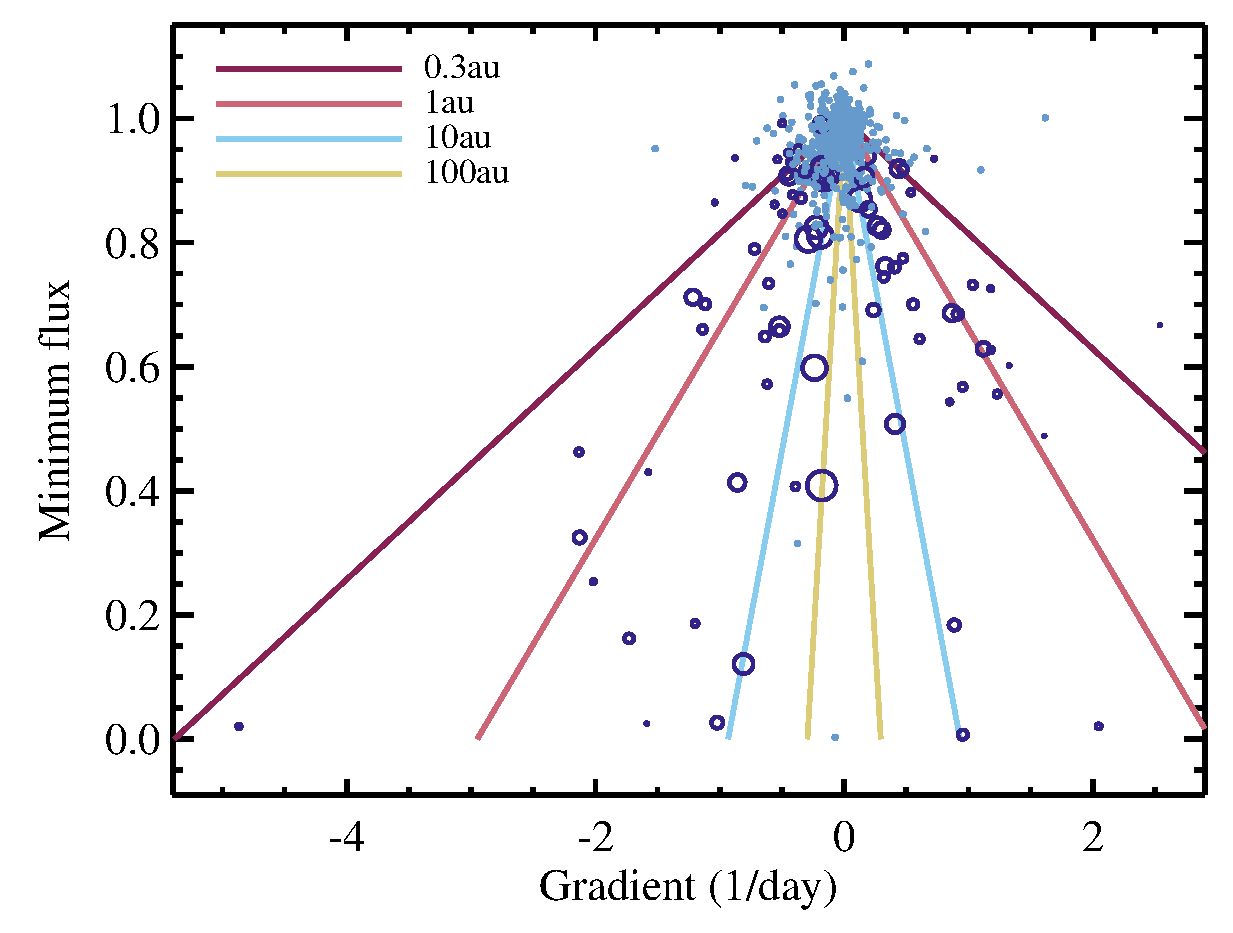
\includegraphics[width=0.5\textwidth]{figs/gradients.eps}
    \caption{Gradient and minimum flux measured from individual nights'
      observations. Open circles have gradients significantly different from zero, and a
      symbol size proportional to the inverse of the gradient uncertainty. Dots are
      consistent with zero slope. The lines show the gradients implied by the velocities
      for circular orbits at 0.3, 1, 10, and 100au.}\label{fig:grad}
  \end{center}
\end{figure}

Using the simple formalism described above, we can use gradients derived directly from
the light curves to estimate the radial location of the occulting clumps. The gradients
are estimated by least squares fitting straight lines to each night's observations, for
which only nights with six or more measurements are used. These gradients are plotted
against the minimum nightly flux $f_{\rm min}$ in Figure \ref{fig:grad}. We plot
gradients whose uncertainty is less than 4$\times$ their value as open circles, with
symbol sizes proportional to the inverse of this uncertainty. All other gradients are
plotted as small dots, as a check that the gradients for unocculted fluxes are near
zero. The horizontal scatter of these gradients near $f_{\rm min}=0$ provides a further
estimate of the uncertainty of individual gradients. The solid lines show the gradients
expected for circular orbits at a range of semi-major axes.

An unusual feature in Figure \ref{fig:grad} is that the gradients may be biased towards
negative values at low $f_{\rm min}$. For the 15 negative, and 4 positive gradients below
$f_{\rm min}=0.5$, and approximately equal numbers of positive and negative gradients
above, Fisher's exact test yields a p-value of 0.02. Thus, there is evidence that the
distributions of gradients above and below minimum fluxes of 0.5 are different, with
negative gradients more commonly seen for deep dimming events. In the range
$0.5<f_{\rm min}<0.8$ there are 15 and 25 negative and positive gradients, a reversal of
the trend, but this difference only has a p-value of 0.1. Thus, there are about equal
numbers of gradients measured with minimum fluxes below 0.8, but their distributions are
different.

The bias to negative gradients below $f_{\rm min}=0.5$ suggests that ingress tends to be
slower than egress; the egress is too quick to be caught. However, the equal numbers
between $0.5 < f_{\rm min} < 0.8$ suggests that the rapid egress does not return the
light curve to quiescence, just to a level above $f_{\rm min}=0.5$. Thus, the statistics
suggest that a typical deep dimming event has an ingress at a rate of $-1$ to $-2$
day$^{-1}$, after which the flux rapidly rises to $f_{\rm min} \approx 0.5$, and then the
remaining egress is at a rate similar to ingress.

Qualitatively, this inference is consistent with a scenario of a disrupted asteroid,
whose structure is dictated by shear and radiation pressure. The fragment size
distribution is such that at least half of the optical depth is contributed by grains
large enough that their orbits relative to the original body are dominated by shear;
forward shearing is more rapid than backward shearing, so the clump has a sharper rear
edge than front edge, accounting for the different number of positive and negative
gradients measured for $f_{\rm min} < 0.5$. The fragments also comprise small grains
whose dynamics are dominated by radiation pressure, which form a ``tail'' much like a
comet's and account for the egress where $f_{\rm min} > 0.5$. We leave the development of
a quantitative study of this scenario for the future, noting that tests of such a model
would require photometry at multiple wavelengths.

A look at specific dimming events shows that such a simple scenario will face challenges,
as shown by the first set of events in 2006 (Figure \ref{fig:waspkeltzoom}); following
the $f \approx 0.5$ dip there are two more nights of data that have higher average
fluxes, but both nights actually have negative gradients. This evolution does not
invalidate the above analysis, but shows that the temporal evolution is complex, and at
any given time multiple clumps, which may or may not be related, could be occulting the
star.

% gradients.pro
\begin{figure}
  \begin{center}
    \hspace{-0.5cm} 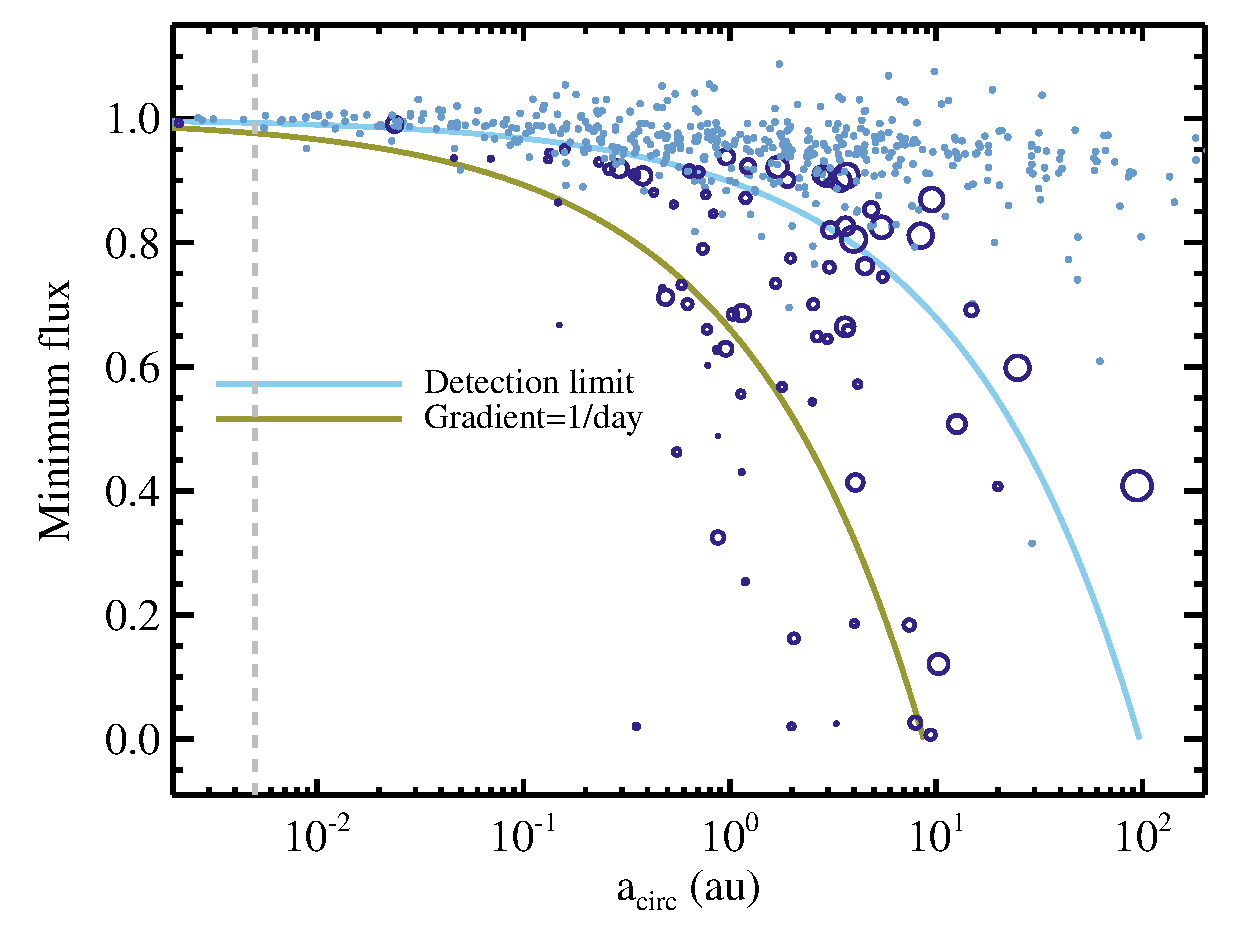
\includegraphics[width=0.5\textwidth]{figs/sma.eps}
    \caption{Semi-major axes estimated from the light curve gradients in Figure
      \ref{fig:grad}. Open circles have gradients significantly different from zero, and
      a symbol size proportional to the inverse of the gradient uncertainty. Dots are
      consistent with zero slope. The stellar radius (grey dashed line) has been
      estimated as Solar. Because gradients may have lower minimum fluxes they can move
      down along lines parallel to the solid lines. Points near or above the blue line
      are consistent with zero light curve gradient.}\label{fig:sma}
  \end{center}
\end{figure}

In Figure \ref{fig:sma} we have converted the gradients into semi-major axes using
equation (\ref{eq:acl}). The dashed line shows the stellar radius, estimated to be
approximately Solar based on an age of 25Myr \citep{2013AstL...39..776P} and an effective
temperature of 5350K \citep{2014A&A...563A.139P} using \citet{2000A&A...358..593S}
isochrones. This Figure also includes solid lines of constant gradient, computed using
equation (\ref{eq:acl}) and $f_{\rm min} = 1-\tau$.

The blue line shows the semi-major axis implied by the scatter in gradients near
$f_{\rm min}=0$ in Figure \ref{fig:grad}. Above this line the gradients can be considered
consistent with zero, and the inferred semi-major axes largely meaningless. A related
point is that because the points near $f_{\rm min}=0$ have very small $\tau$, the derived
velocities and semi-major axes can be rather extreme and should be disregarded. An
additional issue is highlighted by the two large circles near $f_{\rm min}=0.5$ and
between $a_{\rm circ}=30$ to 100, which are the first two nights of 2006 observations
shown in Figure \ref{fig:waspkeltzoom}. The first is at the time of minimum flux, and the
other also appears to be at a turning point, so the assumption behind equation
(\ref{eq:acl}) that $u=0$ (i.e. the cloud edge is passing the stellar disk center) is
clearly incorrect. These points should therefore be associated not with clumps at 30 to
100au, with clumps that lie somewhere interior.

The brown line shows the semi-major axis implied by a gradient of 1/day. As the lowest
flux measured on a given night is not necessarily the minimum flux for that dimming
event, the inferred semi-major axis could be greater; in this case points move downward
parallel to this and similar solid lines. Thus, the main constraint offered by Figure
\ref{fig:sma} is that the clumps orbit with semi-major axes less than 10au.

Figure \ref{fig:sma} suggests that the clumps orbit with projected velocities that are
consistent with circular orbits at about 1au. The conclusion from the IR excess, and
possible the periodicity analysis, is that they may lie closer, near
0.3-0.7au. Reconciling these differences requires that the clumps are on eccentric
obits. For a semi-major axis of 0.3au the minimum clump eccentricity (i.e. all clumps
transit at apocenter) is about 0.6. Such an orientation is of course highly unlikely, so
either the semi-major axis is larger, or the true eccentricities need to be
higher. Perhaps coincidentally, an eccentricity of 0.6 yields a pericenter velocity of
120km s$^{-1}$, similar to the velocity shifts in Sodium absorption lines seen towards
RZ~Psc \citep[][noting however that the pericenter velocity is tangential, and the
absorption lines show projected radial velocity]{2013Ap.....56..453P}.

\subsection{Summary of light curve analysis}\label{ss:wheresum}

The aim of this section was to estimate the location of the bodies that cause the dimming
events towards RZ~Psc. Using ten years of WASP and KELT-North data, we investigated both the
periodicity of possible repeat events, and the light curve gradients. While we found
evidence for a 60-70 day period, this signal is relatively weak. This period would place
the clumps near 0.3au, similar to the distance inferred for the dust seen as an IR excess
(though this location is also uncertain). The gradient analysis places loose constraints
on the clump orbits ($<$10au), so is consistent with a scenario where the clumps have
semi-major axes near 0.3au. Thus, there is no reason to disfavour the model proposed by
\citet{2013A&A...553L...1D}, that the dimming events are associated with clumps being
created by planetesimal collisions within an asteroid belt analogue.

The primary uncertainty lies with the disk evolutionary state. If a significant gas
reservoir remains, a turbulent inner rim scenario similar to that proposed for UXOrs
could produce a similar light curve. Both the lack of accretion, and a likely age beyond
which gas-rich disks are typically seen, may argue against this scenario, though the disk
may be in transition to the debris phase and retain some primordial gas. We revisit the
disk status from the perspective of the flux distribution in section \ref{ss:evol}.

An additional result from the gradient analysis concerns the structure of individual
clumps. The non-uniform gradient distribution is qualitatively consistent with
post-collisional asteroidal fragments being dispersed by a combination of shearing and
radiation pressure. Assuming small dust well-coupled to gas in a hydrodynamic turbulence
scenario, a uniform gradient distribution seems more likely, so we interpret the
gradients as providing circumstantial evidence for the planetesimal fragment scenario.

\section{Disk structure and evolutionary state}\label{s:disk}

Based on ten years of relatively high-cadence photometry, RZ~Psc is regularly occulted by
what are almost certainly star-sized clumps of dust. These clumps can be optically thick,
and previous measurements of colour variations show that at least some of the dust must
be small \citep[e.g.][]{2003ARep...47..580S}, which may be supported by the light curve
gradient statistics. The previous interpretation of this system was that the clumps are
the fragments arising from planetesimal collisions within an asteroid belt analogue that
is also detected in the mid-IR. While the results from the previous section are
consistent with this scenario, the evidence is at best circumstantial as they do not rule
out the alternative of an UXOr-like hydrodynamic inner rim scenario.

We now address several open questions, each taking a slightly wider view. Primary among
these is whether the dimming events and the IR excess are caused by the same dust, as
suggested by \citet{2013A&A...553L...1D}. Two further aspects are then the implications
for the origin of the clumps, the evolutionary status of the disk in which they
reside. We finish by considering the proposed scenarios for dippers and UXOrs, and why
RZ~Psc appears to be a rare object that lies between these classes.

\subsection{Does the occulting dust account for the IR excess?}\label{ss:ir}

One of the reasons that RZ~Psc is worthy of detailed study is that circumstellar dust is
inferred from both the dimming events and the IR excess. Different properties of the dust
grains, and the larger structure in which they reside, are revealed by each method; the
dimming events yield information on dust ``clumpiness'' on a star-sized scale, while the
IR excess provides evidence for an Asteroid belt analogue that captures $\sim$7\% of the
starlight, and thus a measure of the total surface area of dust. The naive expectation is
that the clumps orbit within the asteroid belt, and the dimming events provide therefore
some information on the size distribution and collisional evolution within the belt
\citep{2013A&A...553L...1D}. This expectation however relies on co-location of the clumps
and the belt, for which circumstantial evidence is provided by the light curve gradients
and perhaps the periodicity analysis \citep[see also][]{2010A&A...524A...8G}.

The fraction of starlight intercepted by the dust is a variable common to both the
dimming events and the IR excess. For the former we use the average extinction $\bar{E}$,
which is simply taken from the normalised light curve, as 1 minus the average flux,
yielding 0.05 (the light curve median is 0.995). This estimate assumes that all dimming
events are independent, and the value would be smaller if not since the dust in some
clumps may be being counted two or more times. The lack of strong evidence for
periodicity suggests that multiple counting is not a serious issue however. Another issue
is that the star could be reddened, and therefore that the normalised light curve has
already had some constant level of extinction removed. Based on photospheric colours this
unseen extinction is probably small, in the range of zero to a few percent
\citep{2000ARep...44..611K}.

If we assume that this average extinction applies over a uniform sphere around the star,
and that the dust has a low albedo (i.e. the dimming events are dominated by dust
absorption, not scattering of light out of our line of sight), then the IR fractional
luminosity is equal to the average extinction. That is, both are equal to the fraction of
starlight intercepted by the dust.

To explore possible geometries we use a simple relation between fractional luminosity
$f$, (uniform) geometric optical depth $\tau$, and the disk opening angle $\theta$
\citep{2014MNRAS.tmp...88K}
\begin{equation}
  f = \tau sin(\theta/2) \, ,
\end{equation}
which says that the fractional luminosity is the optical depth of the dust multiplied by
the fraction of the sky covered as seen from the star. The dust belt must therefore have
an opening angle of at least 8$^\circ$ to capture 7\% of the starlight. However, for this
minimal estimate the dust is optically thick, yet RZ~Psc is not seen to be reddened. If
we instead require $\tau \sim \bar{E}$ then as stated in the previous paragraph the dust
distribution must instead be near isotropic.

Given the picture of an asteroid belt analogue and the ubiquity of disk like structures
around young stars, such a spherical distribution seems physically unlikely. It might be
possible to generate a spherical cloud, perhaps by delivery, sublimation, and break-up of
highly inclined comets, as suggested for other warm dust systems such as $\eta$ Corvi
\citep{2007ApJ...658..569W,2012ApJ...747...93L}. Evidence to support this scenario may be
provided by the transient gas absorption seen towards RZ~Psc \citep{2013Ap.....56..453P},
which we discuss further below. We disfavour this scenario primarily because even with
comet scattering, obtaining a spherical distribution of material near the star is
unlikely. Mid-IR interferometry might be able to show that the IR emission originates in
a disk, but the source declination and brightness mean that this test will practically be
difficult.

Thus, the picture of RZ~Psc as a star seen through a \emph{disk}, where the clumps
account for all of the dust and sample some representative part of an asteroid belt
(e.g. the midplane), is untenable because that belt would cause much more reddening than
is observed. These characteristics distinguish RZ~Psc from heavily reddened objects,
where the dimming events could be sampling a more representative section of the disk
\citep[e.g.][]{2015MNRAS.451...26S}. This issue can be avoided by invoking a spherical
distribution of material, but the problem then shifts to whether such a distribution is
physically plausible.

A more likely alternative, which we favour, is that most of the dust does not lie on
orbits that pass in front of the star, and the occultations are caused by a small
fraction of objects that have greater orbital inclinations than average. In this case the
component that causes most of the IR excess may or may not be clumpy, and could be
radially optically thick (i.e. the opening angle could be as small as 8$^\circ$). This
picture unfortunately loses any strong connection between the occulting clumps and the IR
excess, essentially adding a free parameter that is the fraction of material that is
``kicked'' or resides above the disk, but seems to be the simplest and most probable
scenario. \citet{2003ApJ...594L..47D} used essentially the same argument for UXOrs, so
our picture is therefore inevitably similar, at least in terms of geometry, as dust
occultation models proposed for UXOrs
\citep[e.g.][]{1997ApJ...491..885N,2000A&A...364..633N,2003ApJ...594L..47D}.

We therefore conclude that while there is almost certainly some connection between the
dimming events and the IR excess, it is at best indirect; we are (unfortunately) not
viewing RZ~Psc through a representative part of an Asteroid belt analogue. As with other
UXOrs, a clear prediction is that the disk is not seen edge-on, but at an intermediate
inclination.

\subsection{Origin of the occulting structures}\label{ss:orig}

One of the distinguishing characteristics for RZ~Psc is the relatively short duration of
the dimming events $t_{\rm dim}$, which are a few days compared to a few weeks for other
UXOrs \citep[e.g.][]{1999AJ....118.1043H,2010A&A...511L...9C}. If we assume near-circular
orbits at speed $v_{\rm kep}$, $t_{\rm dim}=2(R_{\rm c}+R_\star)/v_{\rm kep}$, where the
clump has radius $R_{\rm c}$.  The clump radius and dimming event duration are related by
\citep[e.g.][]{2016ApJ...816...69A,2016MNRAS.457.3988B}:
\begin{equation}
  R_{\rm cl} \approx 1.85 t_{\rm dim} \, \left( \frac{M_\star}{a} \right)^{1/2} - R_\star \, .
\end{equation}

% We expect that clumps do not survive indefinitely, and expand to become more diffuse with
% time. The expansion means that the duration and depth of a dip depends on when it is
% observed, with the clump optical depth proportional to size $\tau = k R_{\rm cl}^\alpha$,
% where $k$ is a constant, and $\alpha$ contains information on how the clump
% expands. Given a first dimming event with depth $f_{\rm min} = 1-\tau$, further events as
% the clump expands are therefore expected to have depth
% $f_{\rm min} = 1 - k R_{\rm cl}^\alpha$. In the absence of shear, radiation forces, and
% self-gravity all particles would return to exactly the same point in front of the star
% one orbit later, and shear and radiation pressure act only to change when particles
% return, so we expect $\alpha \approx -1$.

% rcl-a.pro
\begin{figure}
  \begin{center}
    \hspace{-0.5cm} 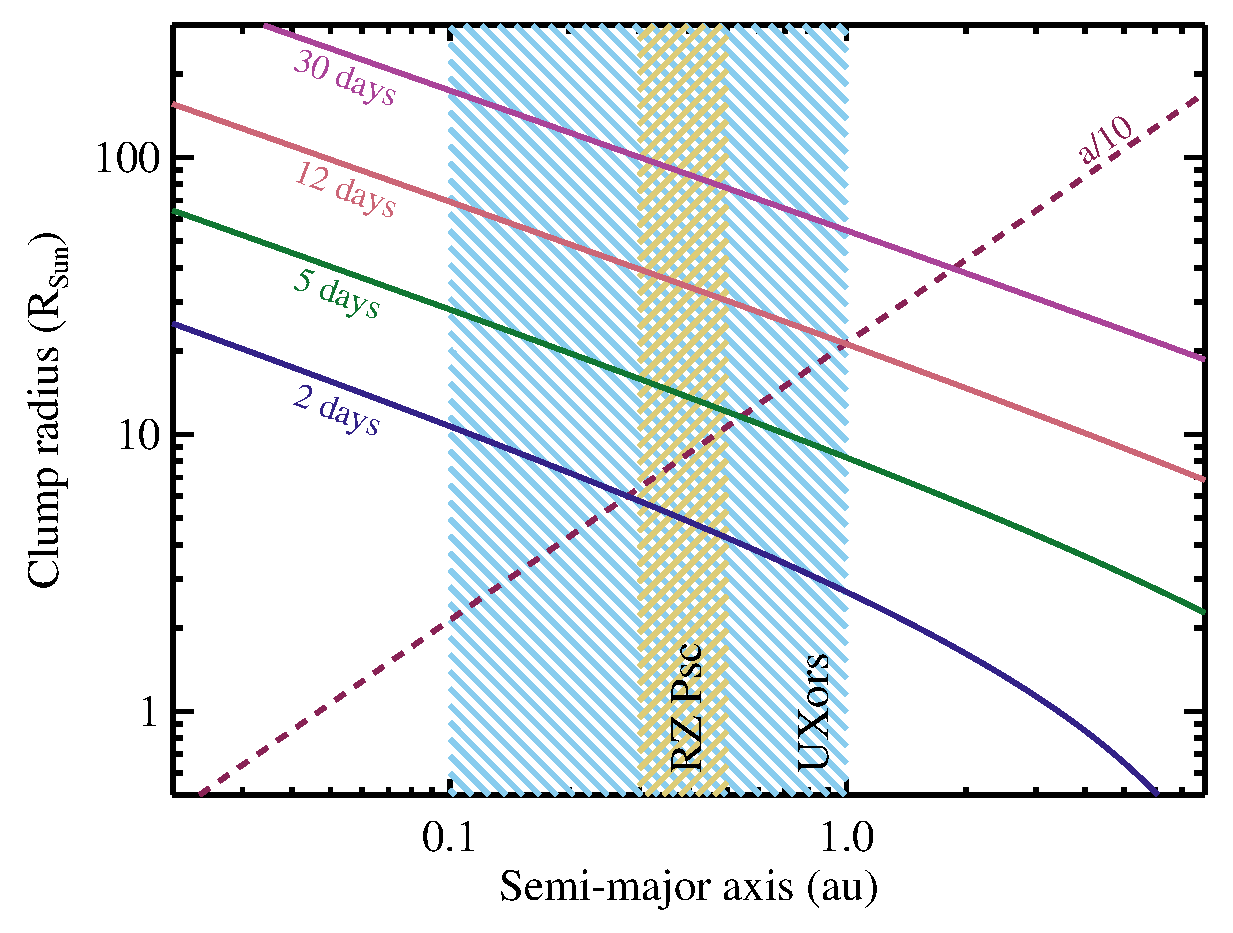
\includegraphics[width=0.5\textwidth]{figs/rcl-a.eps}
    \caption{Clump properties assuming circular orbits for a range of dimming event
      durations (as labelled). The brown region marks the approximate location of the
      RZ~Psc asteroid belt (or the inner edge of a more extended disk). The blue shaded
      region shows a typical Herbig Ae/Be inner disk edge near 1au. The PINK? line shows
      where a clump has an azimuthal extent similar to the scale height of a typical
      gas-rich disk.}\label{fig:rcla}
  \end{center}
\end{figure}

Figure \ref{fig:rcla} shows the radius that clumps must have to cause dimming events of
different durations as a function of semi-major axis. For clumps much larger than the
star the stellar radius is unimportant, and the stellar mass dependence is relatively
weak, so this plot can be applied to RZ~Psc and UXOrs. The radius is of course the
sky-projected size of a clump along the orbit, so whether this scale also applies
vertically and radially depends on the specific scenario. This plot assumes circular
orbits, and that the star has Solar radius and mass. The approximate locations of the
RZ~Psc asteroid belt (or the inner edge of a more extended disk), and the inner edge of a
typical UXOr, are shown by the hatched regions.

The pink line shows where clumps extend a tenth of the semi-major axis - approximately
the scale height for a gas-rich disk. If the variability of both UXOrs and RZ~Psc
originates from dust structures arising from hydrodynamic turbulence, and these
structures are related to the disk scale height, the apparently anomalous short event
durations seen towards RZ~Psc could be explained by the smaller inner disk radius
relative to UXOrs. This suggestion does not rule out hydrodynamic turbulence as an origin
of RZ~Psc's variability nor explain why RZ~Psc is unusual, but shifts the focus to the
disk inner edge. For most UXOrs the inner edge is simply set by sublimation, but for
RZ~Psc the dust could reside much closer than is observed. That is, if the origin of
RZ~Psc's variability is interpreted as similar to other UXOrs, it must host a transition
disk rather than a ``full'' primordial disk. We discuss the evolutionary state of the
disk further below.

A final aspect to discuss regarding the origin of the clumps, and their relation to the
IR excess, is the transient absorption features. These are seen towards UXOrs, but also
seen towards some main-sequence A stars
\citep[e.g.][]{1987A&A...185..267F,2013PASP..125..759W,2014A&A...561L..10K}, so are not
exclusive to stars that host gas-rich disks. For A-type stars these features are
generally interpreted as sun-grazing ``exocomets'', and the same may apply to UXOrs and
RZ~Psc. If these objects can approach the star on isotropically distributed orbits, they
may provide a way for the dimming events to be directly connected to the IR excess (see
section \ref{ss:ir}). A potential issue with this interpretation is that the absorption
lines towards RZ~Psc are so far blue-shifted, and may instead originate in an outflow
\citep{2013Ap.....56..453P}. However, blue-shifting could also occur if evaporation
mostly occurs near periastron passage, which might be expected if the bodies originate in
the asteroid belt and are thus more refractory than the exocomets seen towards other
stars (i.e. an Asteroid in the Solar System would need to pass very close to the Sun to
have a tail). Such a scenario is also consistent with the conclusion of section
\ref{s:where} that the occulting clumps could be on eccentric orbits with high velocities
at periastron. However, an origin closer to the host star makes the likelihood of
isotropic orbits lower. Models of such low-periastron asteroids or comets invariably
require a perturbing planet \citep[e.g.][]{1990A&A...236..202B,1996Icar..120..358B},
which for RZ~Psc would orbit about 2.5 times more distant than the source. That is, if
the asteroid belt is at 0.3au, the planet is near 0.75au. It may be possible that this
planet is inclined and causes the asteroid belt to precess, thus causing the 12.4 year
modulation of the stellar flux seen by \citet{2013A&A...553L...1D}.

\subsection{Disk evolutionary state}\label{ss:evol}

Many young stars with gas-rich disks show broadly similar variability (UXOrs, AA Tau
analogues, dippers). With sporadic and deep photometric minima, and transient absorption
lines, RZ~Psc is most similar to UXOrs and has often been associated with this class,
albeit as a an unusual member \citep[e.g.][]{2010A&A...524A...8G}. Initial distinctions
were made based on the late spectral type (K0V), the relatively short dimming events, and
a lack of near IR excess and accretion signatures. The more recent findings that the
stellar age is probably several tens of Myr, and that the IR excess is suggestive of an
Asteroid belt analogue, further distinguish RZ~Psc as a potentially remarkable object
where the early gas-poor stages of main-sequence debris disk evolution can be
studied. There remain similarities between RZ~Psc and UXOrs. Primarily, we concluded that
the clumps that cause the dimming events are most likely seen when they are well above
the densest regions of a disk, consistent with the turbulent inner rim scenario proposed
by \citet{2003ApJ...594L..47D}.

% sedcomp.pro
\begin{figure}
  \begin{center}
    \hspace{-0.5cm} 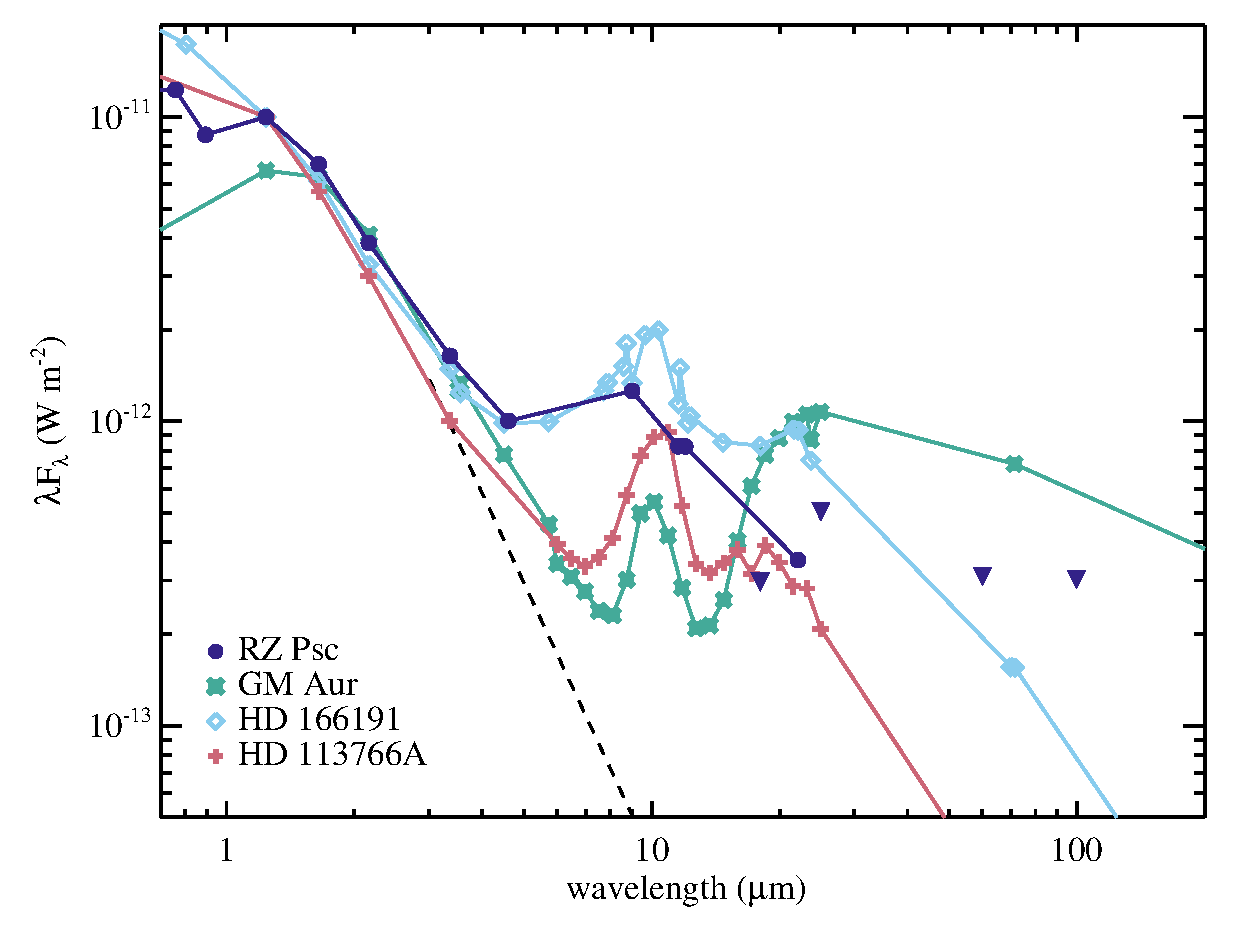
\includegraphics[width=0.5\textwidth]{figs/spcomp.eps}
    \caption{The SED of RZ~Psc in comparison with other young disk-hosting stars. The
      triangles are AKARI and IRAS upper limits for RZ~Psc. Measurements we made at
      different times, so the apparent discrepancy between the WISE detection at 22$\mu$m
      and the AKARI upper limit at 18$\mu$m is probable indicator of IR
      variability.}\label{fig:spcomp}
  \end{center}
\end{figure}

To consider RZ~Psc within a similar framework, Figure \ref{fig:spcomp} shows the spectral
energy distribution (SED) of RZ~Psc, and several other systems that could be considered
to be at a similar evolutionary stage \citep[a similar plot appeared
in][]{2014MNRAS.tmp...88K}. GM Aur hosts a transition disk, the status of HD 166191's
disk is ambiguous and may lie somewhere between the transition and debris phase
\citep{2013arXiv1308.0405S,2014MNRAS.tmp...88K}, and HD 113766A hosts a bright warm
debris disk.

In contrast to UXOrs, there is no obvious reason for dust around RZ~Psc to lie near 0.3
au, as the dust sublimation distance is much closer. For RZ~Psc to host a gas-rich disk
it would therefore probably need to be a transition object that has as-yet undetected
far-IR emission from the outer disk. As illustrated by Figure \ref{fig:spcomp} the limits
set by IRAS are not particularly stringent, but in comparison to GM Aur the flux beyond
20$\mu$m is lower than expected. However, without a mid-IR spectrum for RZ~Psc the level
of the continuum (particularly near 7$\mu$m) and the strength of any 10$\mu$m silicate
feature is unknown, making this comparison difficult. While the lower flux levels beyond
20$\mu$m may suggest that the spectrum is more similar to a debris disk system like HD
113766A, they may arise from self-shadowing of the outer disk \citep[though as noted
by][finding parameters for shadowed outer T~Tauri disks is more difficult than for Herbig
Ae/Be stars]{2003ApJ...594L..47D}.

With the aid of mid-IR interferometry, the disk around HD 113766A has been shown to
comprise two components, one at 0.6 and another at 9au \citep{2013A&A...551A.134O}. This
is by no means evidence that RZ~Psc has a similar structure, but merely reinforces the
fact that the SED does not rule out such possibilities and that the dust need not be
confined to a single belt near 0.3au. Similarly, the disk around HD 166191 was modelled
as an optically thick transition disk extending from 1-25au
\citep{2014MNRAS.tmp...88K}. Thus, it could be that RZ~Psc hosts a disk that extends from
0.3 to a few tens of au, especially if the inner disk is able to shadow the outer
disk. Evidence for shadowing could be sought by searching for the mid-IR ``see-saw''
variability seen towards transition disks \citep[e.g.][]{2009ApJ...704L..15M}.

While the lack of a near-IR excess for RZ~Psc suggests that the disk is at least in the
transition to a debris disk (i.e. has an inner hole), it does not preclude the
possibility that gas resides in that hole and may still be accreting on to the star. No
emission lines that would provide evidence of accretion have been seen
\citep{2013Ap.....56..453P,2014A&A...563A.139P}, but as a further test we constructed the
spectral energy distribution. Specifically, we included photometry from the Galaxy
Evolution Explorer \citep[GALEX,][]{2003SPIE.4854..336M} to quantify the level of any
ultraviolet (UV) excess, a complementary accretion indicator
\citep[e.g.][]{1998ApJ...509..802C}. This exercise is hindered somewhat by the
possibility that optical photometry was obtained when RZ~Psc was not near the quiescent
level. To circumvent this issue we used just the Two Micron All-Sky Survey
\citep[2MASS][]{2003tmc..book.....C} and GALEX photometry, fitting a PHOENIX atmosphere
model \citep{2005ESASP.576..565B}, finding a best-fit effective temperature of 5485K
(assuming no reddening, or 5600K if some reddening is allowed to improve the fit
slightly). These temperatures are consistent with that derived from a high-resolution
spectrum; $5350 \pm 150$K \citep{2014A&A...563A.139P}. Alternatively, fixing the
temperature to the spectroscopic value yields a mild UV excess, less than a factor of
two, that may be chromospheric. We therefore conclude that there is no evidence for
accretion seen as a UV excess

In summary, the status of the disk surrounding RZ~Psc is unclear because the SED is
poorly sampled. Comparison with the infrared spectra of other disks suggests that the
disk is at a minimum well evolved towards the debris phase, and may have reached it
already. This possibility, and the rarity of objects like RZ~Psc, opens the possibility
that it is being observed at a special time with a specific geometry, so may yield better
insights than most systems. A mid-IR spectrum would reveal the strength of any silicate
feature and allow a better comparison with other systems, such as those in Figure
\ref{fig:spcomp}.

\subsection{The rarity of Sun-like dippers/UXOrs}\label{ss:rarity}

% export from cartoon.key, cropped with pdfcrop
\begin{figure}
  \begin{center}
    \hspace{-0.5cm} 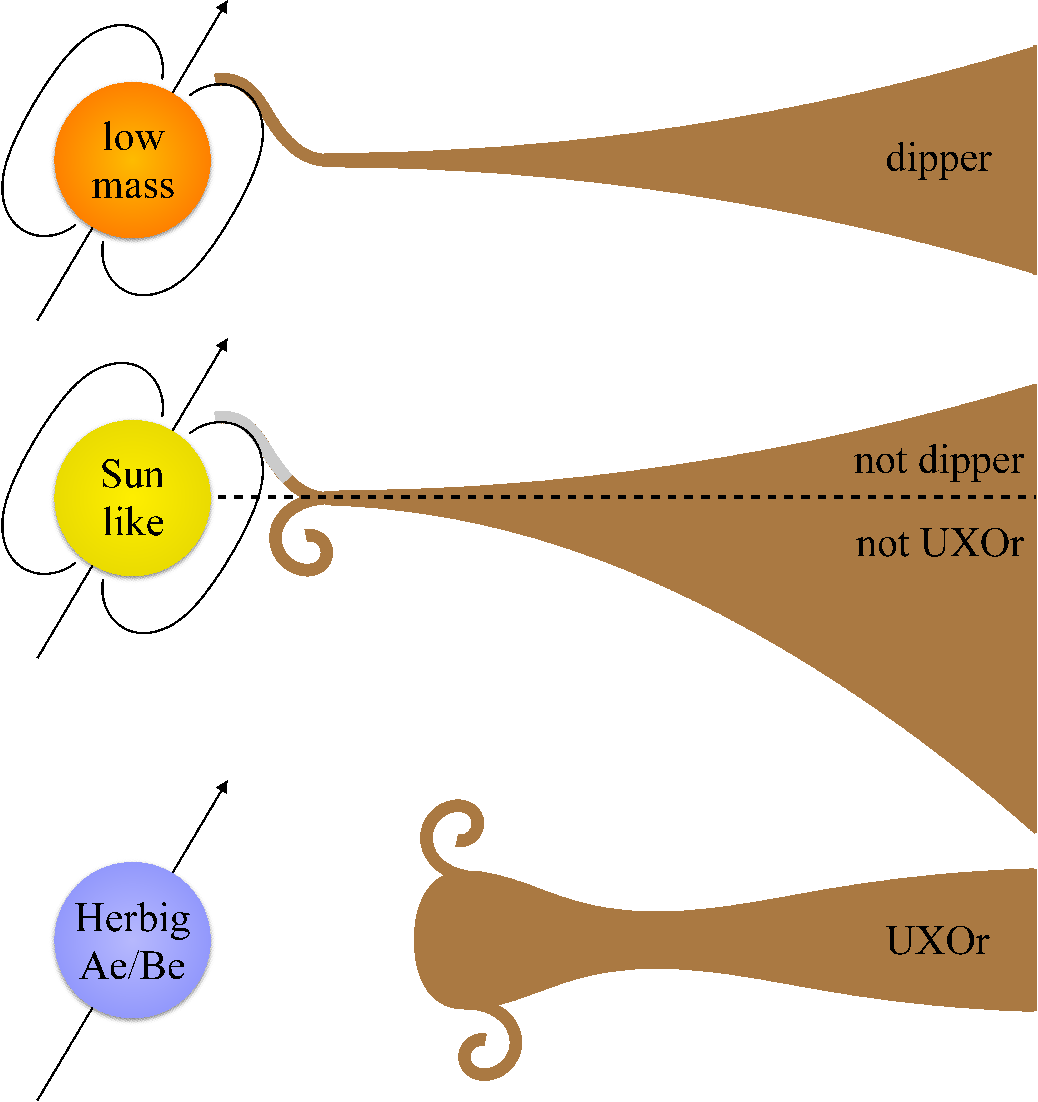
\includegraphics[width=0.5\textwidth]{figs/cartoon-crop.ps}
    \caption{Cartoon showing possible origins of dippers and UXOrs, and why Sun-like
      stars may only rarely show analogous behaviour. In each case the star, magnetic
      dipole, and rotation axis are shown at the left, with possible disk structures
      viewed edge-on to the right. (\emph{top}) low-mass stars (dippers) are occulted by
      co-rotating material that is accreting on to the star, and the dust sublimation
      radius is interior to corotation \citep{2016arXiv160503985B}. (\emph{middle})
      Sun-like stars are rarely seen as dippers or UXOrs because i) dust sublimates
      outside corotation \citep[][represented by the grey accretion column in the upper
      half]{2016arXiv160503985B}, or ii) material lifted by turbulence is shadowed by the
      outer disk (spiral in the lower half). (\emph{bottom}) Herbig Ae/Be stars (UXOrs)
      are occulted by turbulence that appears above self-shadowed disks
      \citep{2003ApJ...594L..47D}. In this type of (primordial) scenario RZ~Psc is
      occulted by turbulence in an evolved disk with little flaring (i.e. dust has
      settled towards the disk midplane).}\label{fig:cartoon}
  \end{center}
\end{figure}

We finish by briefly discussing RZ~Psc in the context of the general classes of dippers
and UXOrs, considering why neither of these classes includes many Sun-like stars like
RZ~Psc. To aid this discussion, Figure \ref{fig:cartoon} shows the proposed scenarios for
dippers and UXOrs, and possible reasons for a lack of significant dust-related dimming
events towards Sun-like stars \citep[see][for similar figures for
dippers]{2016arXiv160503985B}.

From the perspective of dippers, which so far have spectral types later than K5,
\citet{2016arXiv160503985B} explain their tendency to be low-mass stars as a consequence
of the relation between the magnetospheric truncation, corotation, and sublimation
radii. The periodicity of dippers suggests that the occulting material is near the
corotation radius, and is therefore near the base of any accretion columns. For low-mass
stars the dust temperature at this distance is cool enough that the columns contain
significant dust mass and hence the dipping phenomenon is seen (top panel of Figure
\ref{fig:cartoon}. For earlier type stars the sublimation radius is outside the
corotation radius, so any dust in the accretion columns has sublimated and no dipping is
seen (grey accretion column in the middle panel of Figure \ref{fig:cartoon}).

An as-yet unexplored corollary of this scenario is that the outer disks in dipper systems
must not be more flared than the height of the accretion columns (as seen from the
star). This could be because disks around low mass stars are simply less flared in
general \citep[e.g.][]{2010ApJ...720.1668S}, or because disks in dipper systems tend to
be more evolved than average \citep{2016ApJ...816...69A}. Of course, if Sun-like stars
are sufficiently flared that the inner regions are not visible, then whether the
accretion streams are transparent or not is moot.

From the perspective of UXOrs, a possible explanation for their tendency to be B and
A-type stars is that the specifics of self-shadowing are different for Sun-like stars
\citep{2003ApJ...594L..47D}. The reason is unclear, but it seems either that
self-shadowing is simply rarer, or that the nature is different \citep[i.e. shadowing by
the inner disk regions, rather than by a puffed-up inner rim,
see]{2004A&A...421.1075D,2007prpl.conf..555D}

Thus, it seems that the rarity of Sun-like stars among dipper and UXOr populations can be
understood as a result of the scenarios for both. Accretion columns are optically thin
because the dust has sublimated, and any turbulence that rises above the inner disk may
not be seen as it is hidden behind a flaring outer disk.

In this context the rarity of RZ~Psc-like objects can be explained in two ways. The first
simply sidesteps the above discussion by interpreting the disk as a gas-poor asteroid
belt analogue. Examples of such bright disks at a few au are rare
\citep{2013MNRAS.433.2334K}, and only a subset of these will be oriented such that
dimming events are seen (recalling that the occulting bodies are at tens of stellar
radii). The second explanation relies on RZ~Psc's age and SED, which suggest that it
hosts a gas-rich transition disk that is well settled (i.e. not significantly flared),
and hence turbulence above the disk inner edge is visible. The non-detection of RZ~Psc in
the far-IR (Figure \ref{fig:spcomp}) might also be the result of such settling, and
suggests that the brightness at millimeter wavelengths might be brighter than expected
given the mid-IR brightness \citep[e.g.][]{2007prpl.conf..555D}. The rarity is again
explained by an unlikely geometry, and perhaps that the period during which the inner
disk can be seen above the outer disk as it settles is relatively short.

\section{Summary and Conclusions}\label{s:conc}

Long considered a member of the UXOr class of variables, RZ~Psc is almost completely
occulted by dust for several days multiple times during each observing season. The
``typical'' UXOr (which is generally a Herbig Ae/Be object) shows week to month long
dimming events that are thought to be caused by hydrodynamic turbulence above the disk
inner rim, and where the outer disk is self-shadowed \citep{2003ApJ...594L..47D}. Various
anomalous characteristics distinguish RZ~Psc from other UXOrs; the possible age of a few
tens of Myr, the K0V spectral type, the few-day long dimming events, and the location of
the IR-excess emitting dust well beyond the sublimation radius. These characteristics
suggest that RZ~Psc hosts a gas-poor asteroid belt analogue at 0.4-0.7au and that the
dust clumps that occult the star are the dispersed fragments produced in destructive
planetesimal collisions.

To take a critical look at this intriguing scenario, we have presented and analysed ten
years of WASP and KELT-North photometric monitoring of RZ~Psc. We found circumstantial
evidence that some dimming events repeat and have a semi-major axis consistent with that
inferred from the IR excess, but the signal is only significant at the 1-2$\sigma$
level. The light curve gradients are consistent with this picture, but the constraints
are poor. The statistics of the light curve gradients suggest that a typical dimming
event has an egress rate that is initially faster, and then slower, than ingress. While
this evolution seems qualitatively consistent with the structure expected from a
planetesimal collision, quantitative models are needed.

By considering the joint constraints allowed by the light curve and the IR excess, we
find that the objects causing the dimming events are unlikely to be representative of the
structure causing the IR excess. The two can only be reconciled if the IR excess
originates in a spherical shell of clumpy but on average optically thin dust, a scenario
that we cannot rule out but disfavour. Assuming a disk-like structure, the belt is almost
certainly optically thick with an opening angle of a few tens of degrees, with the system
viewed at an inclination that allows clumps residing above this belt to pass in front of
the star. While such a geometry is possible for both UXOr-like and asteroid belt
scenarios, the relatively cool temperature of the dust around RZ~Psc means that if it
hosts a gas-rich disk it must be a transition object. The attraction of such a scenario
is that the dimming event durations could be naturally explained as being shorter than
typical UXOrs simply because the spatial scales at the disk inner edge are smaller for
RZ~Psc.

However, comparison of RZ~Psc's spectrum with other objects suggest that it is more
similar to objects considered to be debris disks, rather than transition disks. This
conclusion in part rests on a low far-IR disk luminosity which could arise if the outer
disk is shadowed (as suggested for UXOrs). The spectrum is poorly sampled and would
benefit from a mid-IR spectrum to better estimate the continuum, and millimeter
photometry to test whether there is a settled outer disk.

Overall, we conclude that the status of RZ~Psc's disk is uncertain, and therefore that so
is the origin of the clumps. The lack of near-IR excess shows that the disk is beyond the
primordial phase, but could be in the final throes of dispersal and the occulting
structures a related phenomenon. Several specific observations would help: i) a mid-IR
spectrum would show the continuum dust level and allow mineralogical comparison with
other systems, and ii) mid-IR spectral monitoring would allow comparisons with transition
disk systems that show ``see-saw'' variability, iii) continuous photometry (ideally with
multiple colours) would yield the detailed shape of individual dimming events and in some
cases the distribution of dust size across the clump.

As a Sun-like star showing disk-related stellar variability, RZ~Psc is a rarity. The
reason may be twofold; i) the sublimation radius is greater than for low-mass stars so
any accretion streams are transparent, and/or ii) in contrast to more massive stars,
turbulence above the inner rim may be shadowed by the outer disk. While the asteroid belt
scenario avoids the need to consider primordial disk structure, in the context of such
models RZ~Psc-like variability could be explained by the evolved state of the disk, which
may have settled enough that the inner rim is visible.

\section*{Acknowledgments}

Data and code used in the preparation of this contribution can be found online at
\href{https://github.com/drgmk/rzpsc}{https://github.com/drgmk/rzpsc}.

We have no competing interests.

GMK initiated the project, collated data, did most of the analysis, and wrote the
paper. MAK contributed early ideas and the iterative event finding method. KGS provided
independent SED models to test for a UV excess. As members of the KELT collaboration, JP,
JER, RJS, and KGS acquired the time-series photometry. All co-authors provided input on
the style and content of the manuscript.

We thank Joachim G\"urtler for sharing photometry from the Sonneberg and Harvard Plates
in a palatable form, AAVSO observers for monitoring RZ~Psc, and Simon Hodgkin and Mark
Wyatt for useful discussions. This paper makes use of data from the DR1 of the WASP data
\citep{2010A&A...520L..10B} as provided by the WASP consortium, and the computing and
storage facilities at the CERIT Scientific Cloud, reg. no. CZ.1.05/3.2.00/08.0144 which
is operated by Masaryk University, Czech Republic.

GMK is supported by the Royal Society as a Royal Society University Research Fellow. MAK
is employed as a lecturer at the Leiden Observatory. JP is employed as a lecturer at
Lehigh University. JER is funded as a Future Faculty Leaders Fellow at the
Harvard-Smithsonian Center for Astrophysics. RS is employed as an Instrumentation
Scientist for the Las Cumbres Observatory Global Telescope Network. KGS is funded as a
lecturer at Vanderbilt University.

\bibliography{../ref} \bibliographystyle{apj}

%\begin{figure*}
\begin{center}
\hspace{-0.25cm} 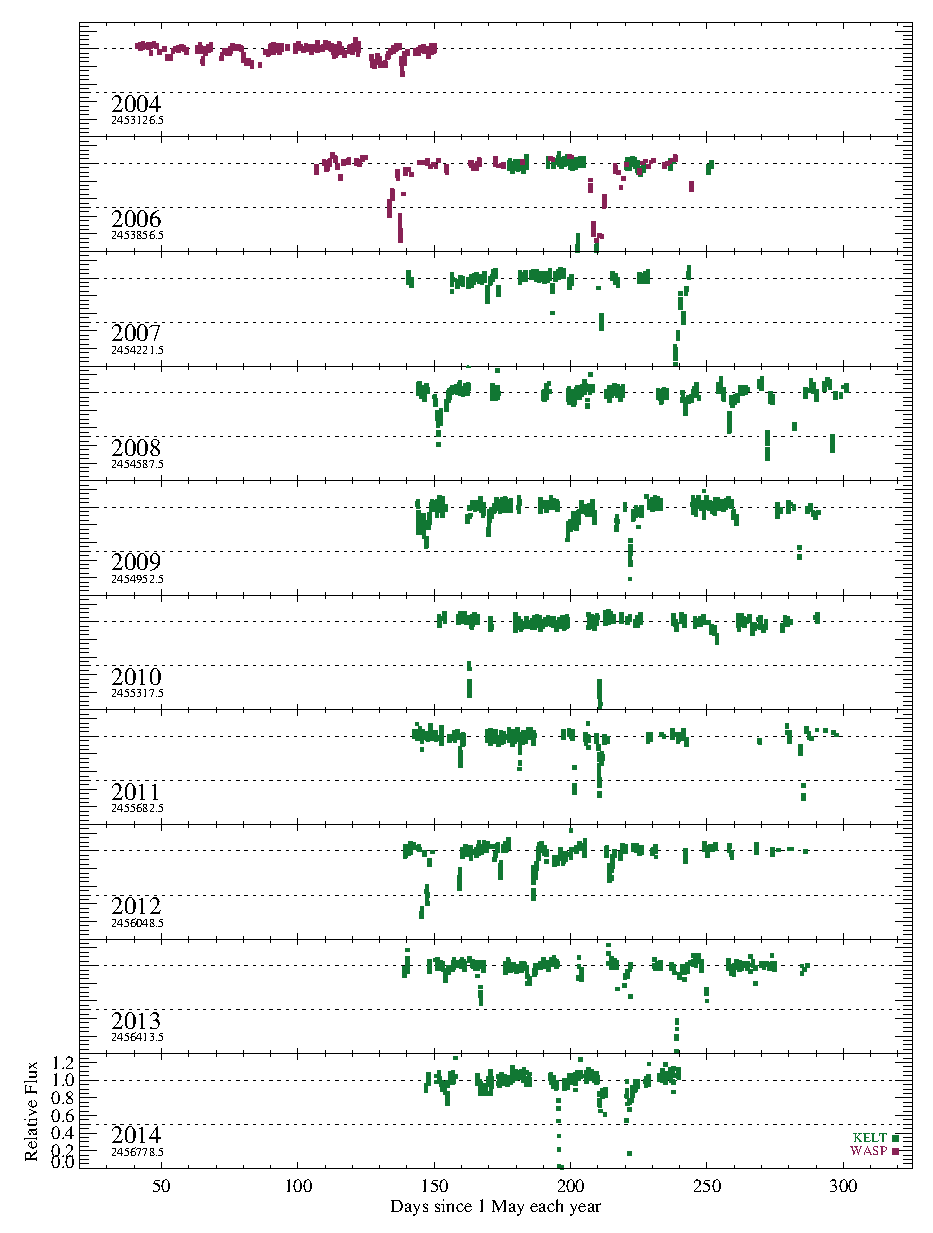
\includegraphics[width=1\textwidth]{figs/yearly-2004.eps}
\caption{V-band photometry for RZ Psc. Rows begin on 1 May of the year shown in each panel, with the initial Julian date also shown.}\label{fig:yearly}
\end{center}
\end{figure*}



\end{document}
